\chapter{Discrete methods in Image Processing}
\label{chapter:discrete-methods-in-image-processing}

In the beginning of the last chapter we described the Bayesian rational for the denoising problem. We turn once again to probability thinking, but restricting our analysis to discrete probabilistic models. Markov Random Fields are in the foundations of the methods discussed in this chapter, and an inspiration for many others. Image pixels are naturally interpreted as Markov states, and image properties, as spatial coherence, are encoded as potentials stored in the edges of the image grid graph. The MAP inference boils down to minimize the challenging class of pseudo-boolean functions. 

In some fortunate cases, the functions can be minimized exactly and efficiently by a reduction to a max-flow (min-cut) problem, and it happens that such cases model imaging problems, as segmentation, nicely well. In fact, the minimum cut defines a partition, and one can interpret the cut as the contour separating two objects. It is the key for fruitful research that has followed. One can abstract the MRF machinery and define potentials on vertices and edges of the grid graph such that its minimum cut answers the problem being posed. Moreover, the potentials can model geometric properties of objects embedded in the grid graph, and one can use cuts to estimate the objects perimeters, for example.

We start this chapter by giving a brief description of Markov Random Fields and the minimization problem arising from the MAP inference. In the second section we present some properties of pseudo-boolean functions and how to optimize them. In the third section we describe the special class of submodular functions and efficient algorithms to compute the minimum of such functions. Finally, we describe successful models in the image processing community based on graph cuts and how one can inject geometric information in them.


\section{Markov Random Fields}
\label{ch2:sec:markov-random-fields}

Let $\mathcal{G}=(\mathcal{V},\mathcal{E})$ an undirected graph with vertices set $\mathcal{V}$ and edges set $\mathcal{E}$. The set of adjacent vertices to $v \in V$ is denoted $\mathcal{N}(v)$. Given two subsets $S,Q \subset \mathcal{V}$, a $(S,Q)$-cut is any subset of edges $\mathcal{E}' \subset \mathcal{E}$ such that $S,Q$ are in different connected components in the graph $\mathcal{G}(\mathcal{V},\mathcal{E} \setminus \mathcal{E}')$. We denote $cut(S,Q)$ the set of all $(S,Q)$ cuts.

For each vertex $v \in \mathcal{V}$ we associate a discrete random variable $X_v$ that take values from a label set $\Gamma_v$ according with some distribution $P$. We group all random variables in vector $\vec{X}$ and we write $\vec{X}_S$ to refer to the set of associated variables with vertex set $S \subset \mathcal{V}$. We also group all the label sets in the collection $\Gamma$. We denote $W_{\vec{X}}$ the set of all configurations for the random vector $\vec{X}$. We say that $\mathcal{H} =(\mathcal{G},\vec{X},\Gamma,P)$ is a \emph{Markov Random Field} (MRF) if for any non-adjacent states $X_u$ and $X_v$, the probability distribution $P$  satisfies the independence conditions below
\begin{align}
	\textbf{Pairwise independencies:}&\quad \Big\{ X_u \perp X_v \;|\; \big\{X_i,\; \forall i \in \mathcal{V}\setminus\{u,v\} \big\}  \Big\} \label{ch2:eq:markov-pairwise-independencies}   \\
	\textbf{Local independencies:}&\quad \Big\{ X_u \perp X_v \;|\; \big\{X_i, \; \forall i \in \mathcal{N}(u)  \big\} \Big\} \label{ch2:eq:markov-local-independencies} \\
	\textbf{Global independencies:}& \quad \Big\{ \vec{X}_S \perp \vec{X}_Q \;|\; \vec{X}_Z,\; \text{where } \vec{X}_Z \in cut(S,Q) \Big\} \label{ch2:eq:markov-global-independencies},
\end{align}
%
where $X_u  \perp  X_v \;|\; \vec{X}_S$ means that variable $X_u$ is independent of $X_v$ given an assignment of variables in $\vec{X}_S$.  For example, the MRF in~\cref{ch2:fig:example-mrf} respects the following expressions 
\begin{align*}
		P\Big(X_1=w_1 \; | \big\{X_i=w_i, \, i \neq 1 \big\} \Big) &= P\Big(X_1=w_1 \; | \; X_2=w_2,X_3=w_3 \Big) \\
		P\Big(X_3=w_3 \; | \big\{X_i=w_i, \, i \neq 3 \big\} \Big) &= P\Big(X_3=w_3 \; | \; X_1=w_1,X_2=w_2, X_4=w_4 \Big) \\
		P\Big(\vec{X}_{C_{123}} = \vec{w} \; | X_4=w_4, X_5=w_5  \Big) &= P\Big(\vec{X}_{C_{123}} = \vec{w} \; | \; X_4=w_4 \Big),		
\end{align*}
%
where we use the shorter notation $\vec{X}_{C_{123}} = \vec{w} $ to denote some assignment of the random variables associated with the nodes of clique $C_{123}$. A clique is any complete subgraph of $\mathcal{G}$. Given a graph, it may be quite difficult to sort out a probability distribution that satisfies~\cref{ch2:eq:markov-pairwise-independencies,ch2:eq:markov-local-independencies,ch2:eq:markov-global-independencies}. However, for the class of MRF that can be \emph{factorized} in terms of the maximal cliques of $\mathcal{G}$, creating a valid probability distribution is straightforward with the help of \emph{clique potential} functions.

\begin{figure}
\center
\begin{minipage}{0.3\textwidth}
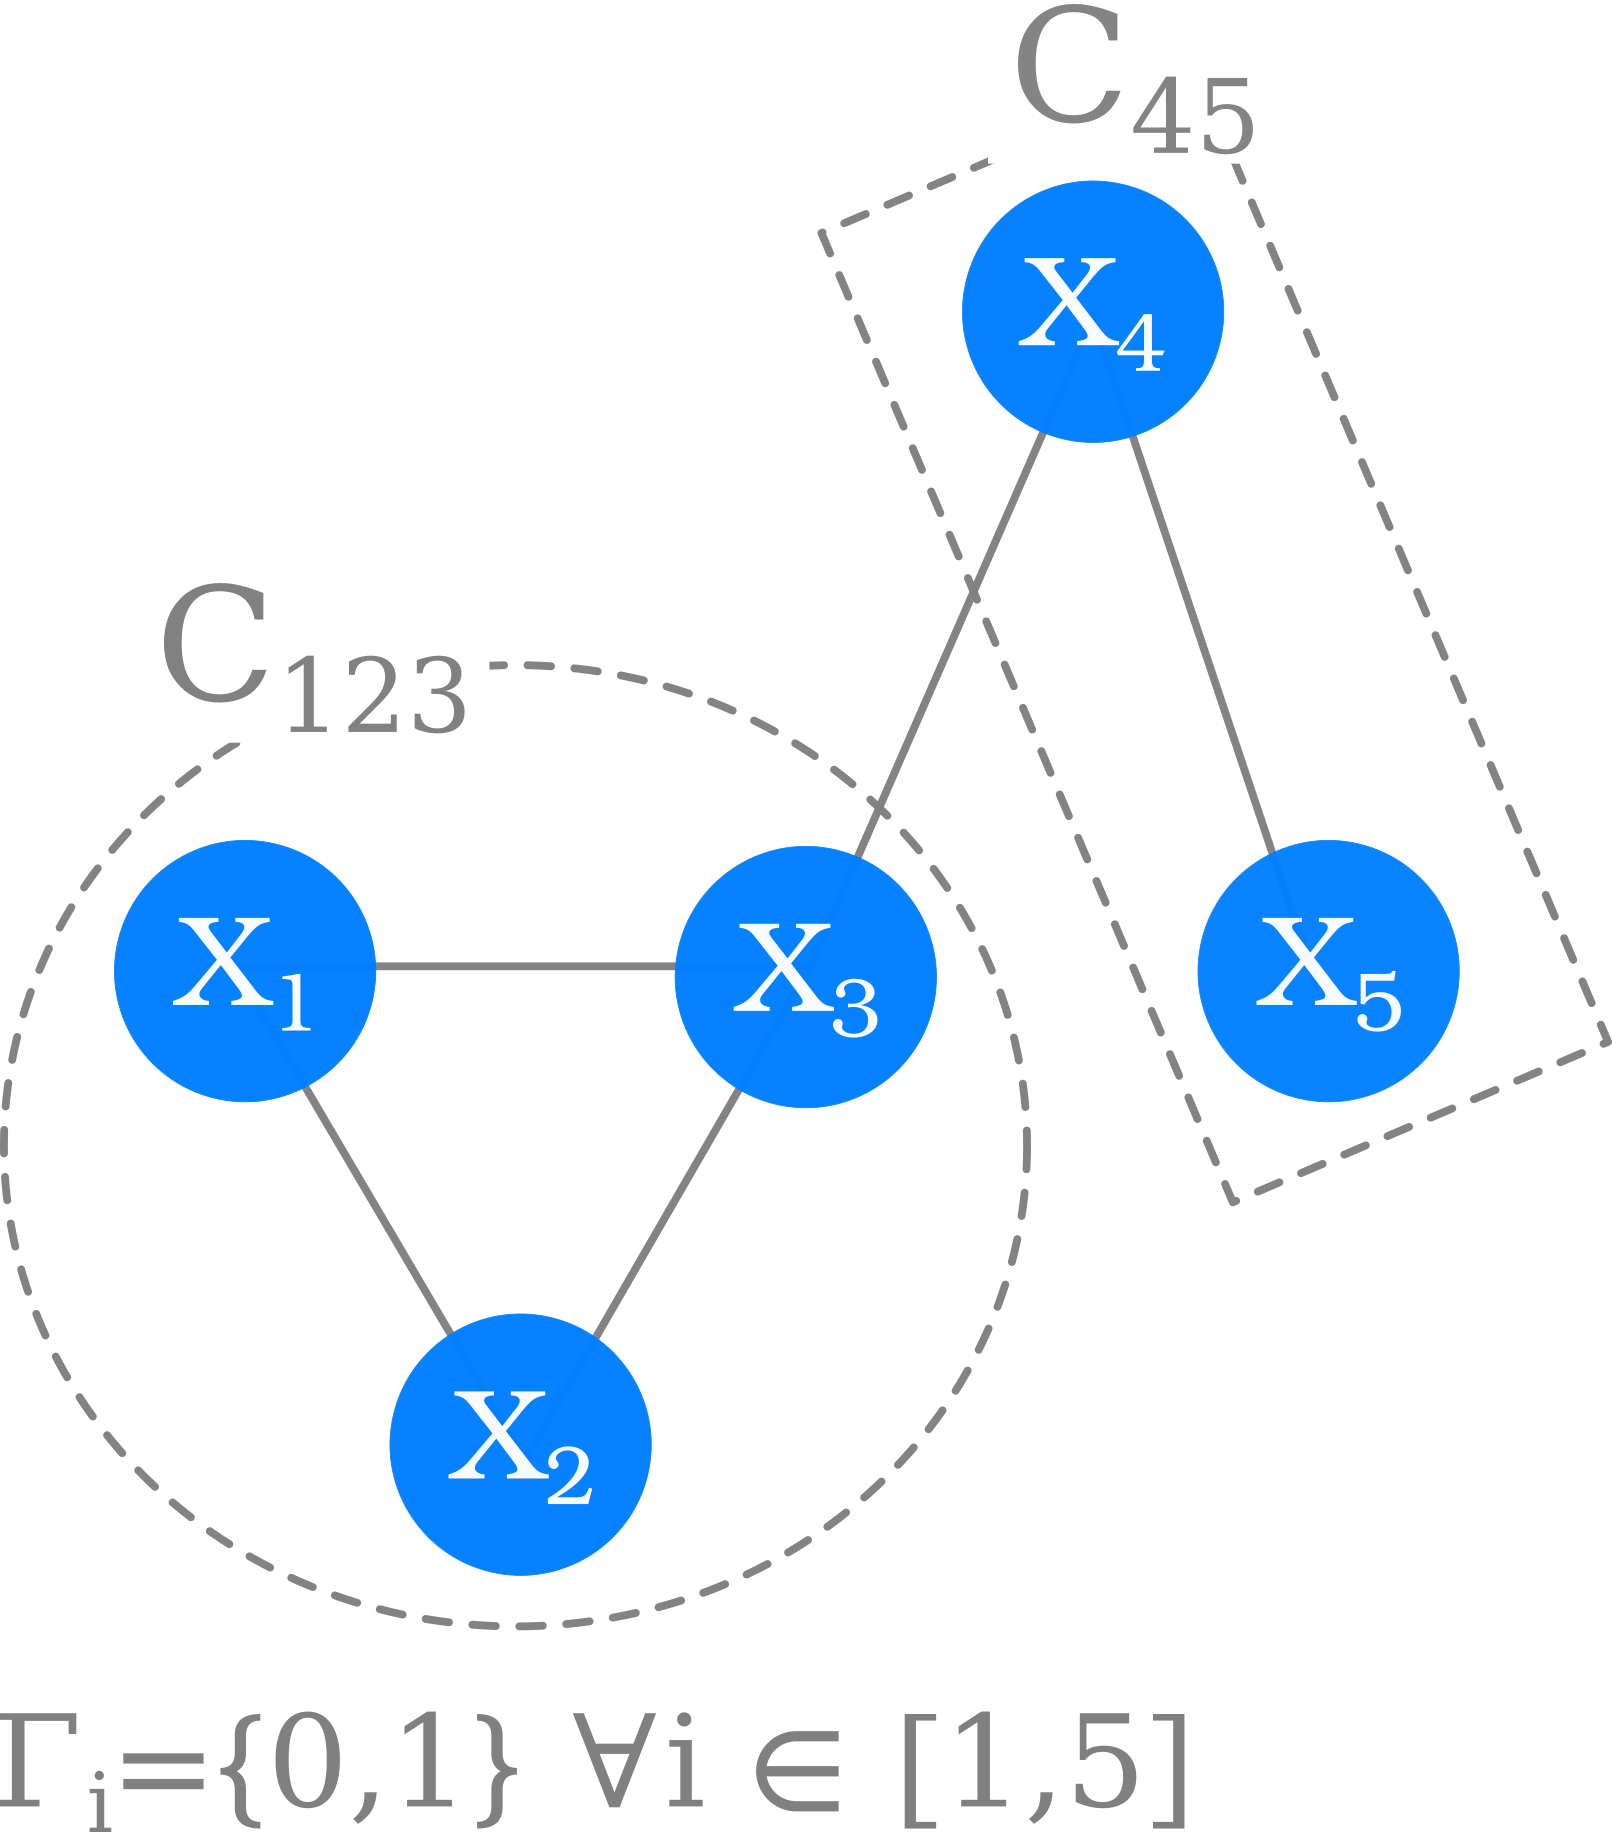
\includegraphics[scale=0.10]{figures/chapter2/mrf/mrf-example.png}
\end{minipage}%
\begin{minipage}{0.35\textwidth}
\tiny
\begin{tabular}{|c|c|c|c|c|l|}
\hline
\multicolumn{5}{|c|}{$\omega$} & \\
\hline
$X_1$ & $X_2$ & $X_3$ & $X_4$ & $X_5$ & $P(\omega)$\\
\hline
0 & 0 & 0 & 0 & 0 & 0.0238 \\
0 & 0 & 0 & 0 & 1 & 0.0023 \\
0 & 0 & 0 & 1 & 0 & 0.0011 \\
0 & 0 & 0 & 1 & 1 & 0.0059 \\
0 & 0 & 1 & 0 & 0 & 0.0238 \\
0 & 0 & 1 & 0 & 1 & 0.0023 \\
0 & 0 & 1 & 1 & 0 & 0.0011 \\
0 & 0 & 1 & 1 & 1 & 0.0059 \\
0 & 1 & 0 & 0 & 0 & 0.119 \\
0 & 1 & 0 & 0 & 1 & 0.0119 \\
0 & 1 & 0 & 1 & 0 & 0.0059 \\
0 & 1 & 0 & 1 & 1 & 0.0297 \\
0 & 1 & 1 & 0 & 0 & 0.0476 \\
0 & 1 & 1 & 0 & 1 & 0.0047 \\
0 & 1 & 1 & 1 & 0 & 0.0023 \\
0 & 1 & 1 & 1 & 1 & 0.0119 \\
\hline
\end{tabular}
\end{minipage}%
\begin{minipage}{0.35\textwidth}
\tiny
\begin{tabular}{|c|c|c|c|c|l|}
\hline
\multicolumn{5}{|c|}{$\omega$} &\\
\hline
$X_1$ & $X_2$ & $X_3$ & $X_4$ & $X_5$ & $P(\omega)$\\
\hline
1 & 0 & 0 & 0 & 0 & 0.119 \\
1 & 0 & 0 & 0 & 1 & 0.0119 \\
1 & 0 & 0 & 1 & 0 & 0.0059 \\
1 & 0 & 0 & 1 & 1 & 0.0297 \\
1 & 0 & 1 & 0 & 0 & 0.0476 \\
1 & 0 & 1 & 0 & 1 & 0.0047 \\
1 & 0 & 1 & 1 & 0 & 0.0023 \\
1 & 0 & 1 & 1 & 1 & 0.0119 \\
\textbf{1} & \textbf{1} & \textbf{0} & \textbf{0} & \textbf{0} & \textbf{0.238} \\
1 & 1 & 0 & 0 & 1 & 0.0238 \\
1 & 1 & 0 & 1 & 0 & 0.0119 \\
1 & 1 & 0 & 1 & 1 & 0.0595 \\
1 & 1 & 1 & 0 & 0 & 0.0952 \\
1 & 1 & 1 & 0 & 1 & 0.0095 \\
1 & 1 & 1 & 1 & 0 & 0.0047 \\
1 & 1 & 1 & 1 & 1 & 0.0238 \\
\hline
\end{tabular}
\end{minipage}
\caption{\textbf{Example of a Markov Random Field}. The nodes $X_1, X_2, X_3$ forms the $3$-clique $C_{123}$.}
\label{ch2:fig:example-mrf}
\end{figure}

\subsection{Clique factorization and Gibbs energy}

A distribution $P_{\Phi}$ is a \emph{Gibbs distribution} if it can be parameterized by a set of factors $\Phi = \{\phi_1,\phi_2,\dots \phi_m\}$, i.e., 
\begin{align*}
	P_{\Phi}(\vec{X} = \vec{w}) &= \frac{1}{Z}\prod_{i=1}^{m}{\phi_i(\vec{w})} \\
	Z &= \sum_{\vec{w} \in W_{\vec{X}}}{ \prod_{i=1}^{m}{\phi_i(\vec{w})} }
\end{align*}
%
%
For strictly positive distributions ($P(\vec{X} = \vec{w}) > 0\; \forall \vec{w} \in W_{\vec{X}}$), the \emph{Hammersley-Clifford} theorem~\cite{koller09} states that $(\mathcal{G},\vec{X},\Gamma,P)$ is a MRF if and only if $P$ is a Gibbs distribution parameterized over complete subgraphs (cliques) of $\mathcal{G}$. Therefore, for MRF with strictly positive distributions $P$ we can write 
\begin{align}
	P(\vec{X} = \vec{w}) &= \frac{1}{Z}\prod_{c \in \mathcal{C}}{\phi_c(\vec{w})} \label{ch2:eq:gibbs-distribution}\\
	Z &=  \sum_{\vec{w} \in W_{\vec{X}}}{ \prod_{c \in \mathcal{C}}{\phi_c(\vec{w})} },\label{ch2:eq:gibbs-constant}
\end{align}
%
where $\mathcal{C}$ is the set of all cliques of $\mathcal{G}$. We define the \emph{order} of such MRF as $\max_{C \in \mathcal{C}} |\mathcal{C}|-1$, i.e., the size of the highest clique in $\mathcal{C}$ minus one. The second order MRF in~\cref{ch2:fig:example-mrf} was constructed by defining the following clique potentials

\begin{center}
\begin{tabular}{ccc}
\begin{tabular}{|c|c|c|c|}
\hline
$X_1$ & $X_2$ & $X_3$ & $\phi_{123}$\\
\hline
0 & 0 & 0 & 1\\
0 & 0 & 1 & 5\\
0 & 1 & 0 & 5\\
0 & 1 & 1 & 10\\
1 & 0 & 0 & 5\\
1 & 0 & 1 & 10\\
1 & 1 & 0 & 10\\
1 & 1 & 1 & 20\\
\hline
\end{tabular}&
\begin{tabular}{|c|c|c|}
\hline
$X_3$ & $X_4$ & $\phi_{34}$\\
\hline
0 & 0 & 100\\
0 & 1 & 50\\
1 & 0 & 20\\
1 & 1 & 10\\
\hline
\end{tabular}&
\begin{tabular}{|c|c|c|}
\hline
$X_4$ & $X_5$ & $\phi_{45}$\\
\hline
0 & 0 & 100\\
0 & 1 & 10\\
1 & 0 & 10\\
1 & 1 & 50\\
\hline
\end{tabular}
\end{tabular}
\end{center}

For strictly positive distributions we also have that the global independencies in~\cref{ch2:eq:markov-global-independencies} are equivalent to the pairwise and local independencies~\cite{koller09}.

\subsection{Hidden Markov model}

Imaging problems are naturally coupled with a set of observations, namely the color intensities of each pixel. We can expect that such observations play a role in any probabilistic model pretending to solve an imaging problem. The \emph{Hidden Markov Model} (HMM) is a subclass of MRF that incorporates such observed variables in its definition and is quite often used in the image processing literature.

\begin{definition}{Hidden Markov Model}
A Hidden Markov Model is a MRF $\mathcal{H} = (\mathcal{G},\vec{X} \cup \vec{Y}, \Gamma_X \cup \Gamma_Y,P)$ such that
\begin{align*}
	Y &= \{ Y_i \; | \; X_i \in \vec{X} \} \\
	\forall i \neq j,& \quad Y_i \perp X_j \; | \; X_i \\
	\forall i \neq j,& \quad Y_i \perp Y_j	.
\end{align*}
\end{definition}
%
We are going to be interested in problems arising from the setting in which the states of random variables in $\vec{Y}$ are known, and one wishes to infer the states of random variables in $\vec{X}$. In other words, we are interest to find $\vec{X}^{\star}$ such that
\begin{align}
	\vec{w}^{\star} &= \argmax_{\vec{w}} = P(\vec{X} = \vec{w} \; | \; \vec{Y}).
%	&= \argmin_{\vec{w}}{E(\vec{w})} \nonumber \\
%	&= \argmin_{\vec{w}}{ \sum_{c \in \mathcal{C}}\sum_{\psi \in \Psi}{\psi(\vec{w}_c})},
	\label{ch2:eq:general-maximum-likelihood}
\end{align}
%
%where $\vec{w}_c$ means the restriction of $\vec{w}$ to its coefficients corresponding to variables in the clique $c$.  
The vector $\vec{Y}$ is called the vector of observed variables, and in image problems they are usually associated to the color intensity of pixels. 

\begin{figure}
\center
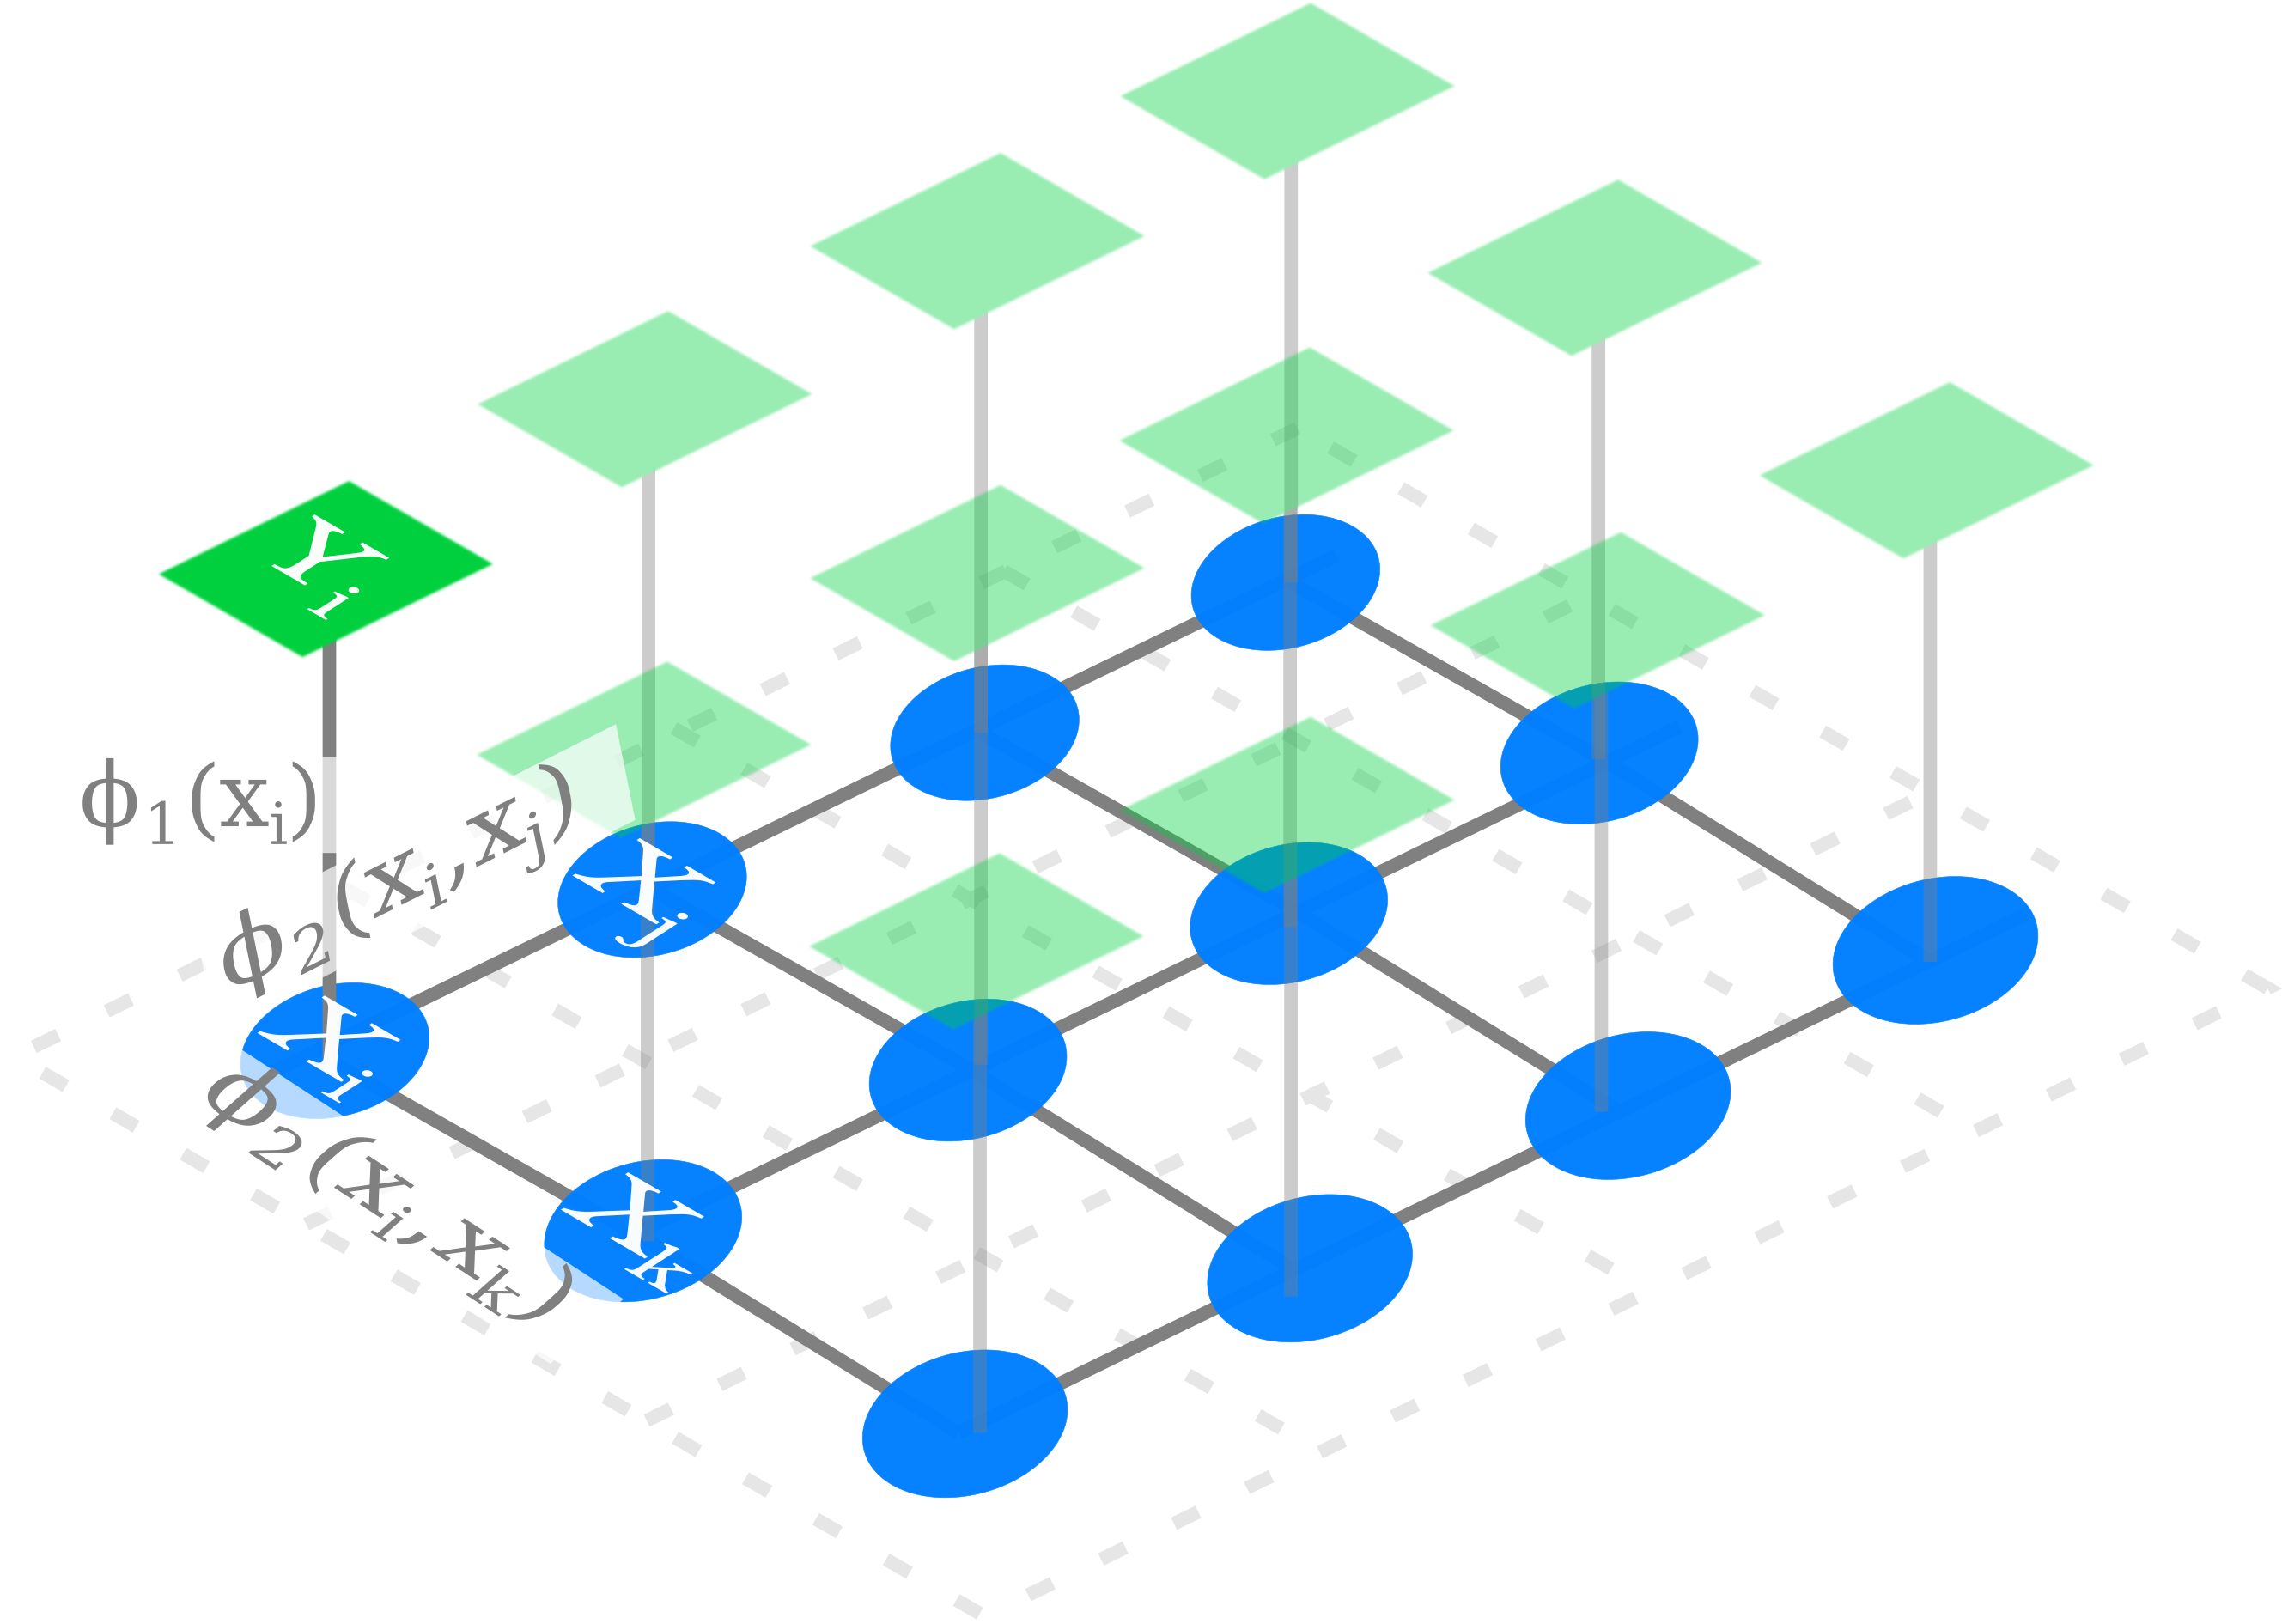
\includegraphics[scale=0.10]{figures/chapter2/mrf/hmm-example.png}
\caption{\textbf{HMM and grid graphs}. A typical HMM in imaging using a $4$-neighborhood system.}
\label{ch2:fig:hmm-multilabeling}
\end{figure}



The set of labels $\Gamma_{\vec{X}}$ is defined according to the problem. In segmentation it could represent the different partitions in which to segment the image, e.g. a label to encode vehicles, another to encode pedestrians, a third to encode the sky and so on. In stereo, the labels could mean the relative depth of the object with respect to the others. In denoising and reconstruction problems in general, it could be the color intensities themselves. 

\subsection{Grid graph and Tikhonov denoising revisited}
Let $\vec{I} \in \mathbb{F}^{m \times n}$ a grayscale bidimensional image. We denote $p \in \vec{I}$ a pixel of $\vec{I}$.  We define its undirected \emph{grid graph} $\mathcal{G}_{\vec{I}}(\mathcal{V},\mathcal{E})$ as
\begin{align*}
	\mathcal{V} &= \{ v_p \; | \; p \in \vec{I} \} \\
	\mathcal{E} &= \big\{ \{v_p,v_q\} \; | \; p \in \vec{I} \text{ and } q \in \mathcal{N}_k(p) \big\},
\end{align*}
%
where $\mathcal{N}_k(p)$ is the $k$-neighborhood of pixel $p$. Common values for $k$ are $4$ and $8$, i.e., 
\begin{align*}
	\mathcal{N}_4(p) &= \{ p + (i,j) \; | \; |i| \leq=1, |j| \leq 1, |i+j|=1 \}\\
	\mathcal{N}_8(p) &= \{ p + (i,j) \; | \; |i| \leq=1, |j| \leq 1 \}.
\end{align*}
%
In the grid graph $\mathcal{G}_I$ we have $1$ and $2$-cliques only. We attach to $\mathcal{G}_I$ the HMM $\mathcal{H} = (\mathcal{G}_I,\vec{X} \cup \vec{Y},\Gamma_{\vec{X}},\Gamma_{\vec{Y}},P)$ in which the random variables take values over the grayscale levels of the image, grouped in $\Gamma_{\vec{X}} = \Gamma_{\vec{Y}} = \{i \; | \; 0 \leq i \leq 255 \}$. The Gibbs distribution $P$ is given by~\cref{ch2:eq:gibbs-distribution,ch2:eq:gibbs-constant} with clique potentials defined as
\begin{equation*}
	\begin{array}{rll}
	\psi_{p}(\gamma_p) &=  \frac{\lambda}{2} \left( f_{\widetilde{\vec{I}}}(p) - \gamma _p \right) ^2. & \\
	\psi_{pq}(\gamma_p, \gamma_q) &= ( \gamma _p - \gamma _q )^2. &\\[1em]
	\phi_p(\vec{x}_p=\gamma _p) &= \exp\big( - \psi_1(\gamma_p) \big),& \quad \forall p \in \vec{I} \\
	\phi_{pq}(\vec{x}_p=\gamma_p, \vec{x}_q=\gamma _q) &= \exp\big( - \psi_{2}(\gamma_p,\gamma_q) \big),& \quad \forall p \in \vec{I} \text{ and }  q \in \mathcal{N}_k(p). \\
	\end{array}
\end{equation*}
%
In~\cref{ch2:fig:hmm-multilabeling} we have a representation of this HMM, which encodes the Tikhonov denoising model of~\cref{ch1:sec:bayesian-rationale}. The estimated image $\widehat{I}$ is computed as the maximum likelihood of $P$, i.e.,
\begin{align}
	\widehat{\vec{I}} &= \argmax_{\vec{I'}}{P(\vec{X}=\vec{I'} \; | \; \vec{Y} = \vec{I} }) \nonumber \\
	&= \argmin_{\vec{I'}}{E(\vec{I'})} \nonumber \\
	&= \argmin_{\vec{I'}}{\sum_{p \in \vec{I}}{\psi_p\big({\vec{I}'(p)}\big)}} + \frac{1}{2}\sum_{ \substack{ p \in \vec{I} \\ q \in \mathcal{N}_k(p)}}{\psi_{pq}\big( {\vec{I}'(p),\vec{I}'(q) \big)}},
	\label{ch2:eq:gibbs-energy-minimization}
\end{align}
%
the $\frac{1}{2}$ factor is necessary in order to compensate double counting of $\psi_{pq}$. The energy $E$ to be minimized is called the \emph{Gibbs energy}.

%\begin{figure}
%\center
%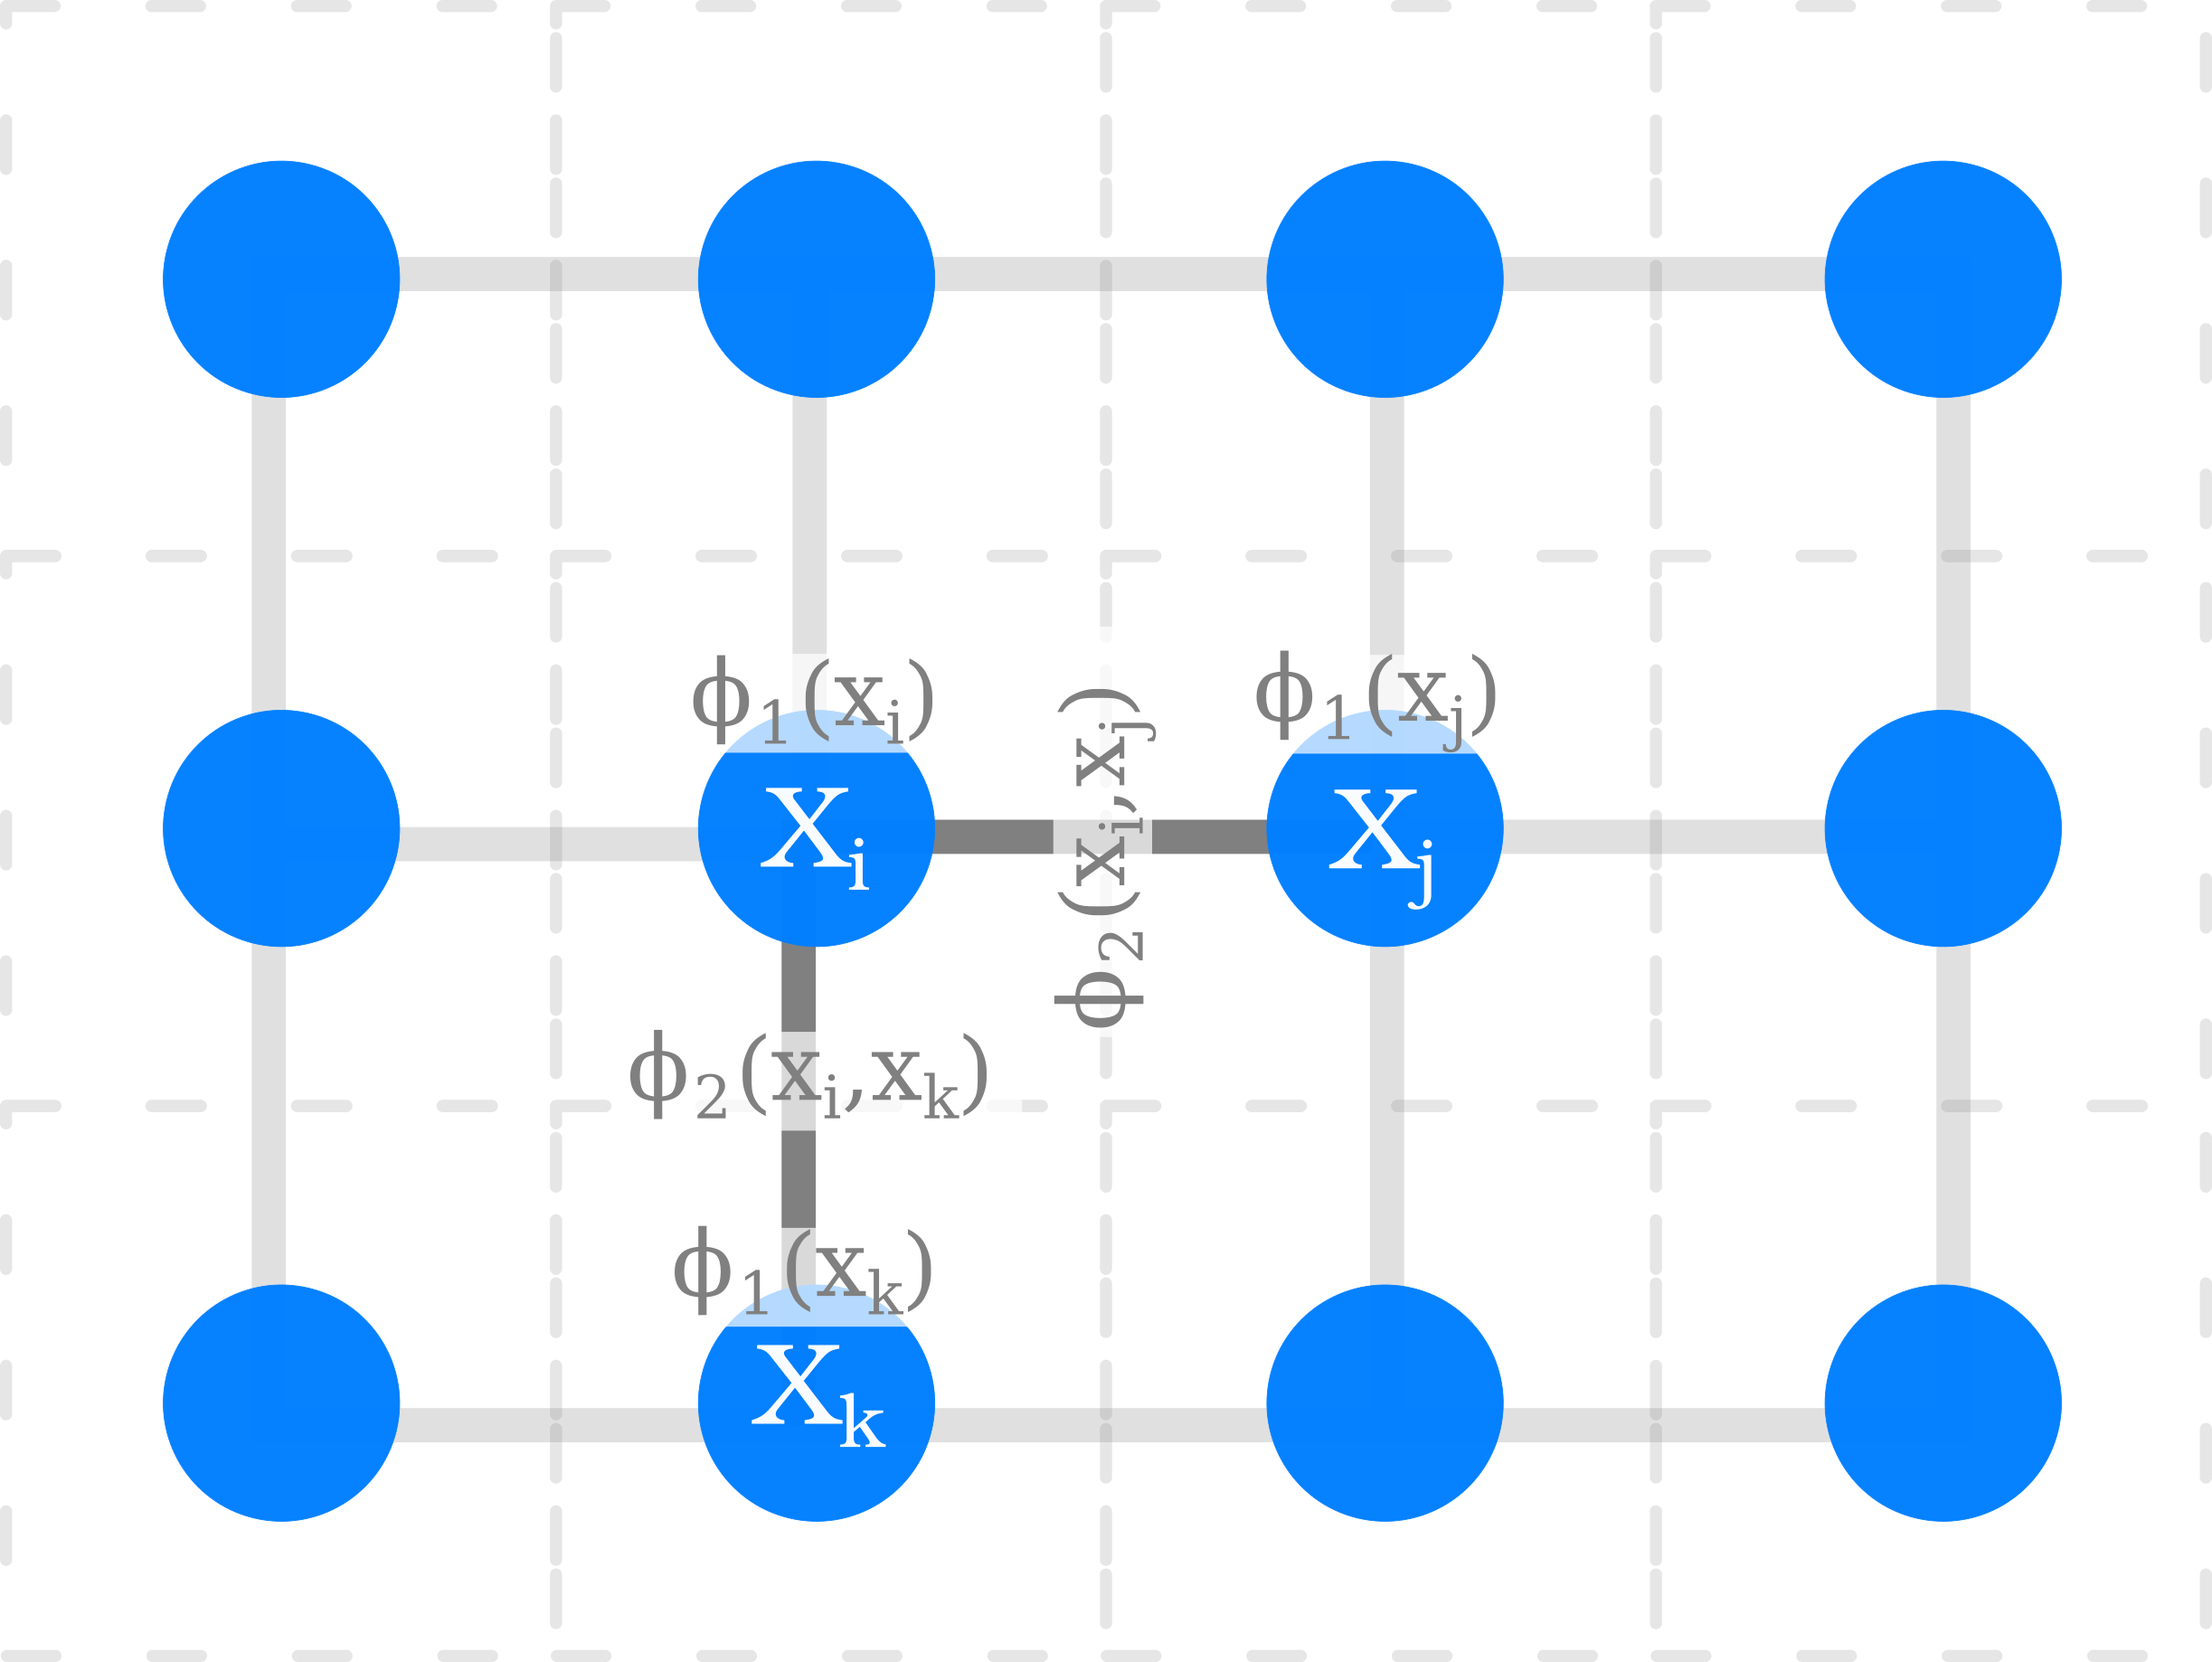
\includegraphics[scale=0.10]{figures/chapter2/grid-graph.png}
%\caption{MRF illustration for Tikhonov image denoising}
%\label{ch2:fig:mrf-tikhonov-denoising}
%\end{figure}


The success of this approach depends on our capacity to minimize the Gibbs energy in~\cref{ch2:eq:gibbs-energy-minimization}. For the Tikhonov multilabel HMM, it can be computed exactly and efficiently~\cite{ishikawa03}. However, MAP inference in general multilabel HMMs is NP-hard. The scenario is a little bit better for binary HMMs, as we are going to see in the next section.

\subsection{Potts and Ising models}

Let $\vec{I} \in \mathbb{F}^{m \times n}$ a grayscale image to which we associated its grid graph $\mathcal{G}_I(\mathcal{V},\mathcal{E})$. We wish to denoise image $\vec{I}$, but instead of using the Tikhonov regularization term, we want to use one that preserves discontinuities. An intermediate step would be to minimize the naive discrete version of total variation, which can also be efficiently minimized. In this case, the Gibbs energy is given by
\begin{align}
	E(\vec{x}) &= \frac{\lambda}{2}\sum_{p \in \vec{I} }{ (\widetilde{I}(p) - x_p)^2} + \sum_{ \substack{ p \in \vec{I}, \\ q \in \mathcal{N}(p) }}{ | x_p - x_q | }.	
	\label{ch2:eq:anisotropic-tv-model-denoising}
\end{align}
%
The term in the right of~\cref{ch2:eq:anisotropic-tv-model-denoising} is called the discrete anisotropic total variation. As its continuous version, the discrete total variation performs better than Tikhonov for imaging problems, but it still not considered a discontinuity preserving function and it presents some undesirable side effects (see~\cref{ch2:fig:comparison-convex-truncated}). On the other hand, truncated functions are discontinuity preserving. For some $K>0$, consider the following Gibbs energy
\begin{align}
	\phi_{pq}(x_p,x_q) &= \left\{ \begin{array}{rl}
		K,& \text{if } x_p \neq x_q \\
		0,& \text{otherwise}.
	\end{array}\right. \label{ch2:eq:potts-model-denoising-1} \\[1em]
	E(\vec{x}) &= \sum_{p \in \vec{I} }{\phi_p(x_p)} + \sum_{\substack{ p \in \vec{I}, \\ q \in \mathcal{N}(p) }}{\phi_{pq}(x_p,x_q)}.	
	\label{ch2:eq:potts-model-denoising-2}
\end{align}
%
~\cref{ch2:eq:potts-model-denoising-1,ch2:eq:potts-model-denoising-2} defines a \emph{Potts model}. Minimizing~\cref{ch2:eq:potts-model-denoising-2} is NP-hard~\cite{boykov01fast} if variables $x_p,x_q$ are not binary, i.e., the underneath HMM is a multilabel one. In the binary case,~\cref{ch2:eq:potts-model-denoising-1,ch2:eq:potts-model-denoising-2} are referred as the \emph{Ising model}, and this one can be minimized efficiently.

\begin{figure}
\center
\subfloat[Noisy image]{
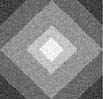
\includegraphics[scale=1.0]{figures/chapter2/convex-and-truncated/noisy-1.png}
}\hspace{1em}
\subfloat[$|x_p - x_q|$]{
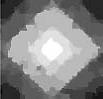
\includegraphics[scale=1.0]{figures/chapter2/convex-and-truncated/absolute-difference-2.png}
}\hspace{1em}
\subfloat[$\min(3, |x_p-x_q|)$]{
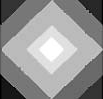
\includegraphics[scale=1.0]{figures/chapter2/convex-and-truncated/truncated-3.png}
}
\caption{\textbf{Comparison between convex and truncated potentials~\cite{blake11markov}(chapter 3)}. Truncated potentials are discontinuity preserving functions, and are suitable for imaging problems.}
\label{ch2:fig:comparison-convex-truncated}
\end{figure}

In fact, MAP inference in multilabel HMMs are much more difficult than MAP inference in binary HMMs. At first glance, the multilabeling extension does not seem to be an issue, as we can always transform a multilabel problem in a binary one by including as many as $\log_2 |\Gamma_{\vec{X}}|$ new variables. The difficulty is that the resulting energy is very likely to lie in a class of binary energies whose minimization is NP-hard~\cite{ramalingam08}. Therefore, MAP inference in multilabel HMMs is not likely to be solved exactly in an efficient manner. Instead, approximation algorithms as $(\alpha,\beta)$-swap~\cite{boykov01fast} or range moves~\cite{veksler07graph} are used.
%(we are going to discuss some of them in~\cref{ch2:sec:graph-cut-models}).

In the next two sections we are going to focus on the analysis of binary first-order HMMs, i.e., MRF that are encoded by $1,2$-cliques potentials and binary random variables. This restriction is justified by two reasons: first because there exist efficient algorithms to solve them (see~\cref{ch2:tab:map-inference-binary-mrf}); and second because of its generality. A general MRF can be transformed into an equivalent binary first-order MRF by including a sufficient number of auxiliary variables. Naturally, such transformations are not always useful. In the multilabel case the derived energy is almost surely non-submodular and in the case of high-order cliques, the inclusion of auxiliary variables may turn the minimization problem impractical~\cite{ishikawa10}.


\begin{table}
\center
\scriptsize
\begin{tabular}{|c|c|m{14em}|m{10em}|}
\hline
\multirow{2}{*}{\textbf{MRF Order}} & \multirow{2}{*}{\textbf{Graph topology}} & \multicolumn{2}{c|}{\textbf{Function class}} \\
\cline{3-4}
&   & \textbf{Submodular} & \textbf{Non-submodular} \\
\hline
$0^{th}$ order & All topologies & \multicolumn{2}{c|}{Greedy algorithm} \\
\hline
\multirow{2}{*}{$1^{st}$ order} & $1$-connected & \multicolumn{2}{m{24em}|}{Viterbi algorithm~\cite{viterbi67}, Belief Propagation~\cite{pearl82}} \\
\cline{2-4}
& $\geq 2$-connected & Max-Flow: $\scriptstyle O(|V|^2|E|)$~\cite{kolmogorov04whatenergies} & \multirow{2}{=}[-2mm]{NP-Hard~\cite{nemhauser81}} \\
\cline{1-3}
$2^{nd}$ order & All topologies & Max-Flow: $\scriptstyle O(|V|^2|E|)$~\cite{billionnet85} & \\
\cline{1-3}
Higher order & All topologies & $O(n^5Q + n^6)$~\cite{orlin09faster} & \\
\hline
\end{tabular}
\caption{\daniel{\textbf{MAP inference algorithms for binary MRF of different orders}}. In $0^{th}$ order HMM, a simple Greedy algorithm computes the MAP inference. In $1^{st}$ order HMM we have linear algorithms based on dynamic programming for $1$-connected graphs and max-flow for other topologies. For orders greater than $2$, MAP inference can be computed efficiently if the $2$-clique potential is submodular. Notice, however, that the best algorithm for orders greater than $2$ is quite expensive ($Q$ denotes the time to evaluate the function). Submodular functions is a special class of Pseudo-Boolean functions discussed in~\cref{ch2:sec:pseudo-boolean-functions} that can be minimized in polynomial time, in constrast with non-submodular, which in this case is proven to be a problem in NP-hard. There are other classes of pseudo-boolean functions that are efficiently optimized, some of them are described in~\cite{boros02pseudo}   }
\label{ch2:tab:map-inference-binary-mrf}
\end{table}


%We are going to restrict our investigation in the next two sections to the general class of binary MRFs, noticing that a multilabel MRF can always be transformed into an equivalent binary one~\cite{ramalingam08} by including a sufficient number of additional states. We remark, however, that such strategy may not be the most efficient, and a couple of multilabeling methods are presented in~\cref{ch2:sec:graph-cut-models}.

%In binary first-order MRFs, the clique potentials maps binary vectors to real values, i.e., the clique potentials are \emph{pseudo-boolean} functions. It can be shown that any pseudo-boolean function can be transformed into an equivalent quadratic pseudo-boolean function~\cite{ishikawa10}, i.e., each term involves at most two binary variables. Therefore, to optimize~\cref{ch2:eq:general-maximum-likelihood} it is sufficient to know how to optimize expressions of type


In binary first-order MRFs, the clique potentials maps binary vectors to real values and the energy belongs to the class of \emph{quadratic pseudo-boolean} functions, which can be written as
\begin{align*}
	f(x_1,\cdots, x_n) &= \sum_{j < n}{c_jx_j} + \sum_{j<k<n}{c_{jk}x_jx_k}.
\end{align*} 
%
In the next section, we explore the class of pseudo-boolean functions and how to optimize them.

\section{Pseudo-boolean functions}
\label{ch2:sec:pseudo-boolean-functions}

\begin{definition}{Pseudo-boolean function}
	A pseudo boolean function $f:\{0,1\}^n \rightarrow \mathbb{R}$ is a function that maps binary vectors to real values.
\end{definition}

Pseudo-boolean functions (PBF) can be interpreted as \emph{set functions}, i.e., functions that map sets to real values. Indeed, a binary vector of $n$ elements is in bijection with the power sets of $V = \{1,2,\cdots,n\}$. Therefore, the PBF $f:\{0,1\}^n \rightarrow \mathbb{R}$ can be written as
\begin{align}
	f(x_1,\cdots,x_n) &= \sum_{S \subset 2^{V}}{c_S \prod_{i \in S}{x_i}}.
	\label{ch2:eq:pbf-polynomial-form}
\end{align}
%
where $c_S \in \mathbb{R}$ is a coefficient associated to each subset $S$. ~\cref{ch2:eq:pbf-polynomial-form} is denoted the \emph{polynomial form} of PBF $f$. The \emph{order} of a PBF is defined as the cardinality of the largest subset $S$ in which $c_S>0$. The polynomial form is \textbf{unique}. 

Sometimes it is convenient to express $f$ in its so called \emph{posiform} representation, usually denoted by $\phi$ instead of $f$. In its posiform representation we use literals $x_i,\bar{x}_i \in L$  to represent states $1,0$ of indexed variable $i$ and all coefficients are positive except the one associated to the empty set.
\begin{align}
	\phi(f) = \phi(x_1,\cdots,x_n) &= \sum_{T \subset 2^{L}}a_T{\prod_{p \in T}{p}},
\end{align}
%
where $a_T \geq 0$ whenever $T\neq \emptyset$. The posiform representation can be seen as a truth table with positive values for all configurations, except the one in which all variables are set to zero. One can pass from posiform to polynomial representation by exchanging $\bar{x}_i$ and $(1-x_i)$. A posiform is said \emph{maximum-constant}  if its constant term $C(\phi)$ is maximum among all posiforms representing $f$. A maximum-constant posiform is denoted $\phi^{\star}$. Both general and maximum-constants posiforms are \textbf{not unique} representations of the PBF $f$.

\begin{example}The polynomial form and two possible posiform representations for the same PBF.
\begin{align*}
	f(x_1,x_2) &= a_{\emptyset} + a_\ol{1} + a_\ol{2} + a_\ol{12} + \big(a_1 - a_\ol{1} + a_{1\ol{2}} - a_\ol{12}\big)x_1 \\
	&+ \big(a_{2} - a_\ol{2} + a_{\ol{1}2} - a_{\ol{12}}\big)x_2\\ 
	&+ \big(a_{12} - a_{\ol{1}2} - a_{1\ol{2}} + a_{\ol{12}}\big)x_1x_2 \\[1em]
	\phi_1(x_1,x_2) &= a_{\emptyset} + a_1x_1 + a_\ol{1}\ol{x_1} + a_2x_2 + a_\ol{2}\ol{x_2} \\ 
			&+ a_{12}x_1x_2 + a_{\ol{1}2}\ol{x_1}x_2 + a_{1\ol{2}}x_1\ol{x_2} + a_{\ol{12}}x_1\ol{x_2} \\[1em]			
	\phi_2(x_1,x_2) &= (a_{\emptyset}-c) + (a_1+c)x_1 + (a_\ol{1}+c)\ol{x_1} + a_2x_2 + a_\ol{2}\ol{x_2} \\ 
			&+ a_{12}x_1x_2 + a_{\ol{1}2}\ol{x_1}x_2 + a_{1\ol{2}}x_1\ol{x_2} + a_{\ol{12}}x_1\ol{x_2} 	
\end{align*}
\end{example}
%
Classical problems in combinatorial optimization as vertex cover, maximum independent set, $3$-SAT and many others are formulated as PBF optimization problems. The mentioned problems are in NP-complete, so we can expect that the optimization of a general PBF is a task that is unlikely to be solved efficiently. Nonetheless, we can investigate subclasses of PBF in which the optimum can be found efficiently.

\subsection{PBF optimization}
 We first observe that optimizing a PBF of order $n$ can be transformed into an equivalent quadratic PBF optimization problem by creating extra variables and penalty terms. For example, let $x,y,w,z \in \{0,1\}$. Then,
 \begin{align*}
 	z=xy \leftrightarrow  xy -2xz-2yz+3x=0 \\
 	z \neq xy \leftrightarrow  xy -2xz-2yz+3x>0
 \end{align*}
%
 Therefore
\begin{align*}
	\min f(x,y,w) &= \min g(x,y,w,z) \\
    \min xyw &= \min zw + xy -2xy -2yz +3x .
\end{align*} 
%
  This procedure can be extended and formally described in a polynomial time algorithm that transforms an arbitrary PBF $f$ in a quadratic PBF $g$ with the property that $\min f = \min g$~\cite{boros02pseudo}. We remark, however, that the transformation may add a prohibitive number of auxiliary variables, turning the minimization problem impractical. With that in mind, we are going to restrict our analysis to the optimization of quadratic PBFs.
  
\subsubsection{Roof duality}

A quite natural and naive approach to optimize~\cref{ch2:eq:pbf-polynomial-form} would be to formulate the quadratic PBF as a continuous linear programming. Consider the quadratic PBF
\begin{align}
	f(\vec{x}) = \left\{ \begin{array}{rl}
		\min &c_0 + \sum_{}{c_ix_i} + \sum_{}{c_{ij}x_ix_j} \\
	\text{subject to }& \vec{x} \in \{0,1\}^n.
	\end{array}\right.
	\label{ch2:eq:qpbf-qip-formulation}
\end{align}
%
~\cref{ch2:eq:qpbf-qip-formulation} can be linearized by substituting each pairwise term $x_ix_j$ with binary variable $z_{ij}$ and including the following set of constraints 
\begin{align*}
	R(\vec{x},\vec{z}) &= \left\{  \begin{array}{l}
	z_{ij} \leq x_i, \\
	z_{ij} \leq x_j, \\
	z_{ij} \geq x_i + x_j - 1 
	\end{array} \Bigg|\; \forall 0<i<j<n \right\}
\end{align*}
%
Therefore, an equivalent linear integer programming formulation is
\begin{align}
	\begin{array}{rl}
		\min& c_0 + \sum_{}{c_ix_i} + \sum_{}{c_{ij}z_{ij}} \\
		\text{subject to }&  \vec{x},\vec{z} \in \{0,1\}^n\\
		&R(\vec{x},\vec{z})	
	\end{array}
	\label{ch2:eq:qpbf-lp-formulation}
\end{align}
%
Finally, the relaxation of~\cref{ch2:eq:qpbf-lp-formulation} gives
\begin{align*}
	g(\vec{x},\vec{z}) &= \left\{ \begin{array}{rl}
		\min& c_0 + \sum_{}{c_ix_i} + \sum_{}{c_{ij}z_{ij}} \\
		\text{subject to }&  \vec{x},\vec{z} \in [0,1]^n\\
		&R(\vec{x},\vec{z})
	\end{array}\right.
\end{align*}
%
Clearly, formulation $G$ is a lower bound of $f$, i.e.,  $g(\vec{x},\vec{z}) \leq f(\vec{x})$. Such lower bound is called the \emph{roof dual} (it was originally defined for a maximization problem) and it is shown~\cite{hammer84} to be equivalent to
\begin{align*}
	g(\vec{x},\vec{z}) &= C_{\phi^{\star}(f)},
\end{align*}
%
i.e., the constant in the max-constant posiform representation of $f$. In this same work, the so called \emph{strong persistency} theorem is proven. It says that for every unary term $a_pp$ ($p$ a literal) in a max-constant posiform representation of $f$, we have that $p=0$ in every solution of $\min f$.
%
\begin{example}
Consider the quadratic PBF 
\begin{align*}
	f(x_1,x_2,x_3) &= 6-x_1-4x_2-x_3+3x_1x_2+x_2x_3.
\end{align*}
%
It can be shown that its roof dual equals $2$. A possible max-constant posiform representation for $f$ is
\begin{align*}
	\phi^{\star}(f) &= 2 + x_1 + \bar{x}_2 + x_1x_2 +2\bar{x}_1\bar{x}_2 + \bar{x}_2\bar{x}_3
\end{align*}
%
According with the strong persistency theorem, $x_1=0,\bar{x}_2=0$ for every solution of $\min f$. Replacing this values in $f$ we have
\begin{align*}
	\min f(x_1,x_2,x_3) &=\min f(x_1=0,\bar{x}_2=0,x_3) \\
	&= \min 6 - 4 - x_3 + x_3 \\
	&= 2.
\end{align*}
\end{example}
%
The strong persistency theorem allow us to fix some variables of the quadratic PBF, which could possibly result in a simpler optimization problem. Clearly, the main difficult is to find the max-constant posiform $\phi^{\star}(f)$ that results in a maximum number of variable elimination. Such posiform, called the \emph{master posiform}, can be found by computing the maximum flow in some capacitated graph.

\subsubsection{Master posiform and max-flow reduction}

We present a construction given in~\cite{boros91,boros02pseudo} of a capacitated graph $G_{\phi}(\mathcal{V},\mathcal{E},c)$ that encodes some posiform $\phi$ with constant $C(\phi)=0$. The authors showed how to derive the max-constant posiform from the computation of the maximum flow of $G_{\phi}$. Let $\phi$ be a posiform of the form
	\begin{align*}
		\phi &= \sum_{p \in L}{a_pp} + \sum_{p,q \in L}{a_{pq}pq},
	\end{align*}
%
with $a_p >0, a_{pq}>0\; \forall p,q \in L$	. We  construct the capacitated graph $G_{\phi}(\mathcal{V},\mathcal{E},c)$ such that each term in the sum is encoded by two edges. Each unary term with literal $p$ have one edge from the source $s$ to its negated literal vertex $v_{\bar{p}}$ and one edge from $v_p$ to the target vertex $\bar{s}$. The source and target vertices are identified with the $1$ and $0$ constants, respectively. 

\begin{center}
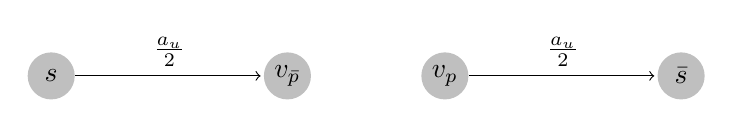
\begin{tikzpicture}[shorten >=1pt,->]
  \tikzstyle{vertex}=[circle,fill=black!25,minimum size=17pt,inner sep=0pt]

  \node[vertex] (G-s) at (0,0) {$s$};
  \node[vertex] (G-np) at (3,0) {$v_{\bar{p}}$};  
  \draw (G-s) -- (G-np) node[midway,above] {$\frac{a_u}{2}$};
    
  \node[vertex] (G-p) at (5,0) {$v_{p}$};    
  \node[vertex] (G-ns) at (8,0) {$\bar{s}$};      
  \draw (G-p) -- (G-ns) node[midway,above] {$\frac{a_u}{2}$};
  
\end{tikzpicture}
\end{center}

Similarly, pairwise terms with literals $p,q$ have edges $\edge{v_p}{v_{\bar{q}}} $ and $\edge{v_q}{v_{\bar{p}}}$. The full graph is given by
\begin{align*}
	\mathcal{V} =& \{ v_p \; | \; p \in L \} \cup \{s,\bar{s}\} \\[1em]
	\mathcal{E} =& \big\{ \edge{s}{v_{\bar{p}}},\edge{v_p}{t} \; | \; \forall a_p>0 \big\} \cup \big\{ \edge{v_p}{v_{\bar{q}}}, \edge{v_q}{v_{\bar{p}}} \; | \; \forall a_{pq} > 0 \big\}  \\[1em]
	c(\, (v_p,v_q)\, ) = c_{pq} =& \left\{ \begin{array}{rl}
		a_{p}/2, & \text{if } v_p \notin \{s,\bar{s}\} \text{ or } v_q \notin \{s,\bar{s}\} \\
		a_{pq}/2, & \text{if } v_p,v_q \notin \{s,\bar{s}\}\\ 
		0,& \text{otherwise}.
	\end{array}\right.
\end{align*}
%
A construction of graph $G_{\phi}$ is illustrated in~\cref{ch2:fig:posiform-capacitated-graph-a}. Therefore, the posiform $\phi$ can also be written as $\phi = \sum_{ \edge{v_p}{v_q} \in \mathcal{E}}{ c_{p\bar{q}} }$. In fact, it is possible to show that there is a bijection between the posiform with zero constant $\phi$ and the graph $G_{\phi}$.


A flow is a function $\varphi:\mathcal{E}\rightarrow \mathbb{R}_{+}$ that satisfies
\begin{equation*}
	\begin{array}{rll}
	\displaystyle
	\varphi(\,\edge{v_p}{v_q}\,) = \varphi (p,q) <& c_{pq},&  \forall v_p,v_q \in \mathcal{V} \\[1em]
	\displaystyle
	\sum_{v_p \in \mathcal{V}}{\varphi(p,q)} =& \displaystyle \sum_{v_p \in \mathcal{V}}{\varphi (q,p)}, & \forall v_q \in \mathcal{V}.	
	\end{array}
\end{equation*}
%
A flow $\varphi ^{\star}$ is said to be maximum if 
\begin{align*}
	\varphi ^{\star} &= \argmax_{\varphi} \sum_{v_p \in \mathcal{V}}{\varphi(s,v_p)},
\end{align*}
%
i.e., if the flow leaving the source is maximum. The residual graph of $G_{\phi}$ with respect to some flow $\varphi$ is denoted $G_{ \phi [ \varphi ] }(\mathcal{V},\mathcal{E}^+,r)$ and owns the same set of vertices of $G_{\phi}$. The set of edges is extended to include returning edges as well, i.e.,
\begin{align*}
	\mathcal{E}^+ &= \mathcal{E} \cup \{ \edge{v_q}{v_p} \; | \; \edge{v_p}{v_q} \in \mathcal{E} \}.
\end{align*}
%
The edges cost is given by the residual function $r$
\begin{align*}
	r(\, \edge{v_p}{v_q} \, ) = r_{pq} &= \left\{ \begin{array}{ll}
	c_{pq} - \varphi( p,q ), & \edge{v_p}{v_q} \in \mathcal{E}\\
	\varphi( p,q ), & \edge{v_p}{v_q} \in \mathcal{E}^+ \setminus \mathcal{E}.
\end{array}\right.	 
\end{align*}
%
One can also construct a posiform from the residual graph $G_{ \phi [ \varphi ] }$. In this case, the posiform is denoted $\phi_{G_{ \phi [ \varphi ] }}$. We remark that edges arriving in the source or leaving the target are all mapped to $0$, as the source and the target are identified with the constants $1,0$ respectively. For example, $\edge{p}{s}$ is encoded as $p\bar{s}=0$.

The \emph{Ford-Fulkerson} algorithm computes the maximum flow by incrementing an initial zero flow function $\varphi_0=0$ every time an \emph{augmenting path} is found. The $k$-th augmenting path is a path $\pi_k = (p_0=s,p_1,p_2,\cdots,p_n,p_{n+1}=\bar{s})$ in the residual graph $G_{ \phi [\varphi_{k-1}] }$ in which all edges of $\pi_k$ have a positive residual value. We say that $\pi_k$ is an $\epsilon$-augmenting path if 
\begin{align*}
	\epsilon = \min_{p_i \in \pi_k\setminus {\bar{s}}} r_{p_i,p_{i+1}}.
\end{align*}
%
\begin{figure}
\center
\subfloat[Initial graph $G_{\phi}$ for $\phi = 2x + 8z + 2x\bar{z} + 4\bar{x}y + 6\bar{y}\bar{z}$\label{ch2:fig:posiform-capacitated-graph-a}]{
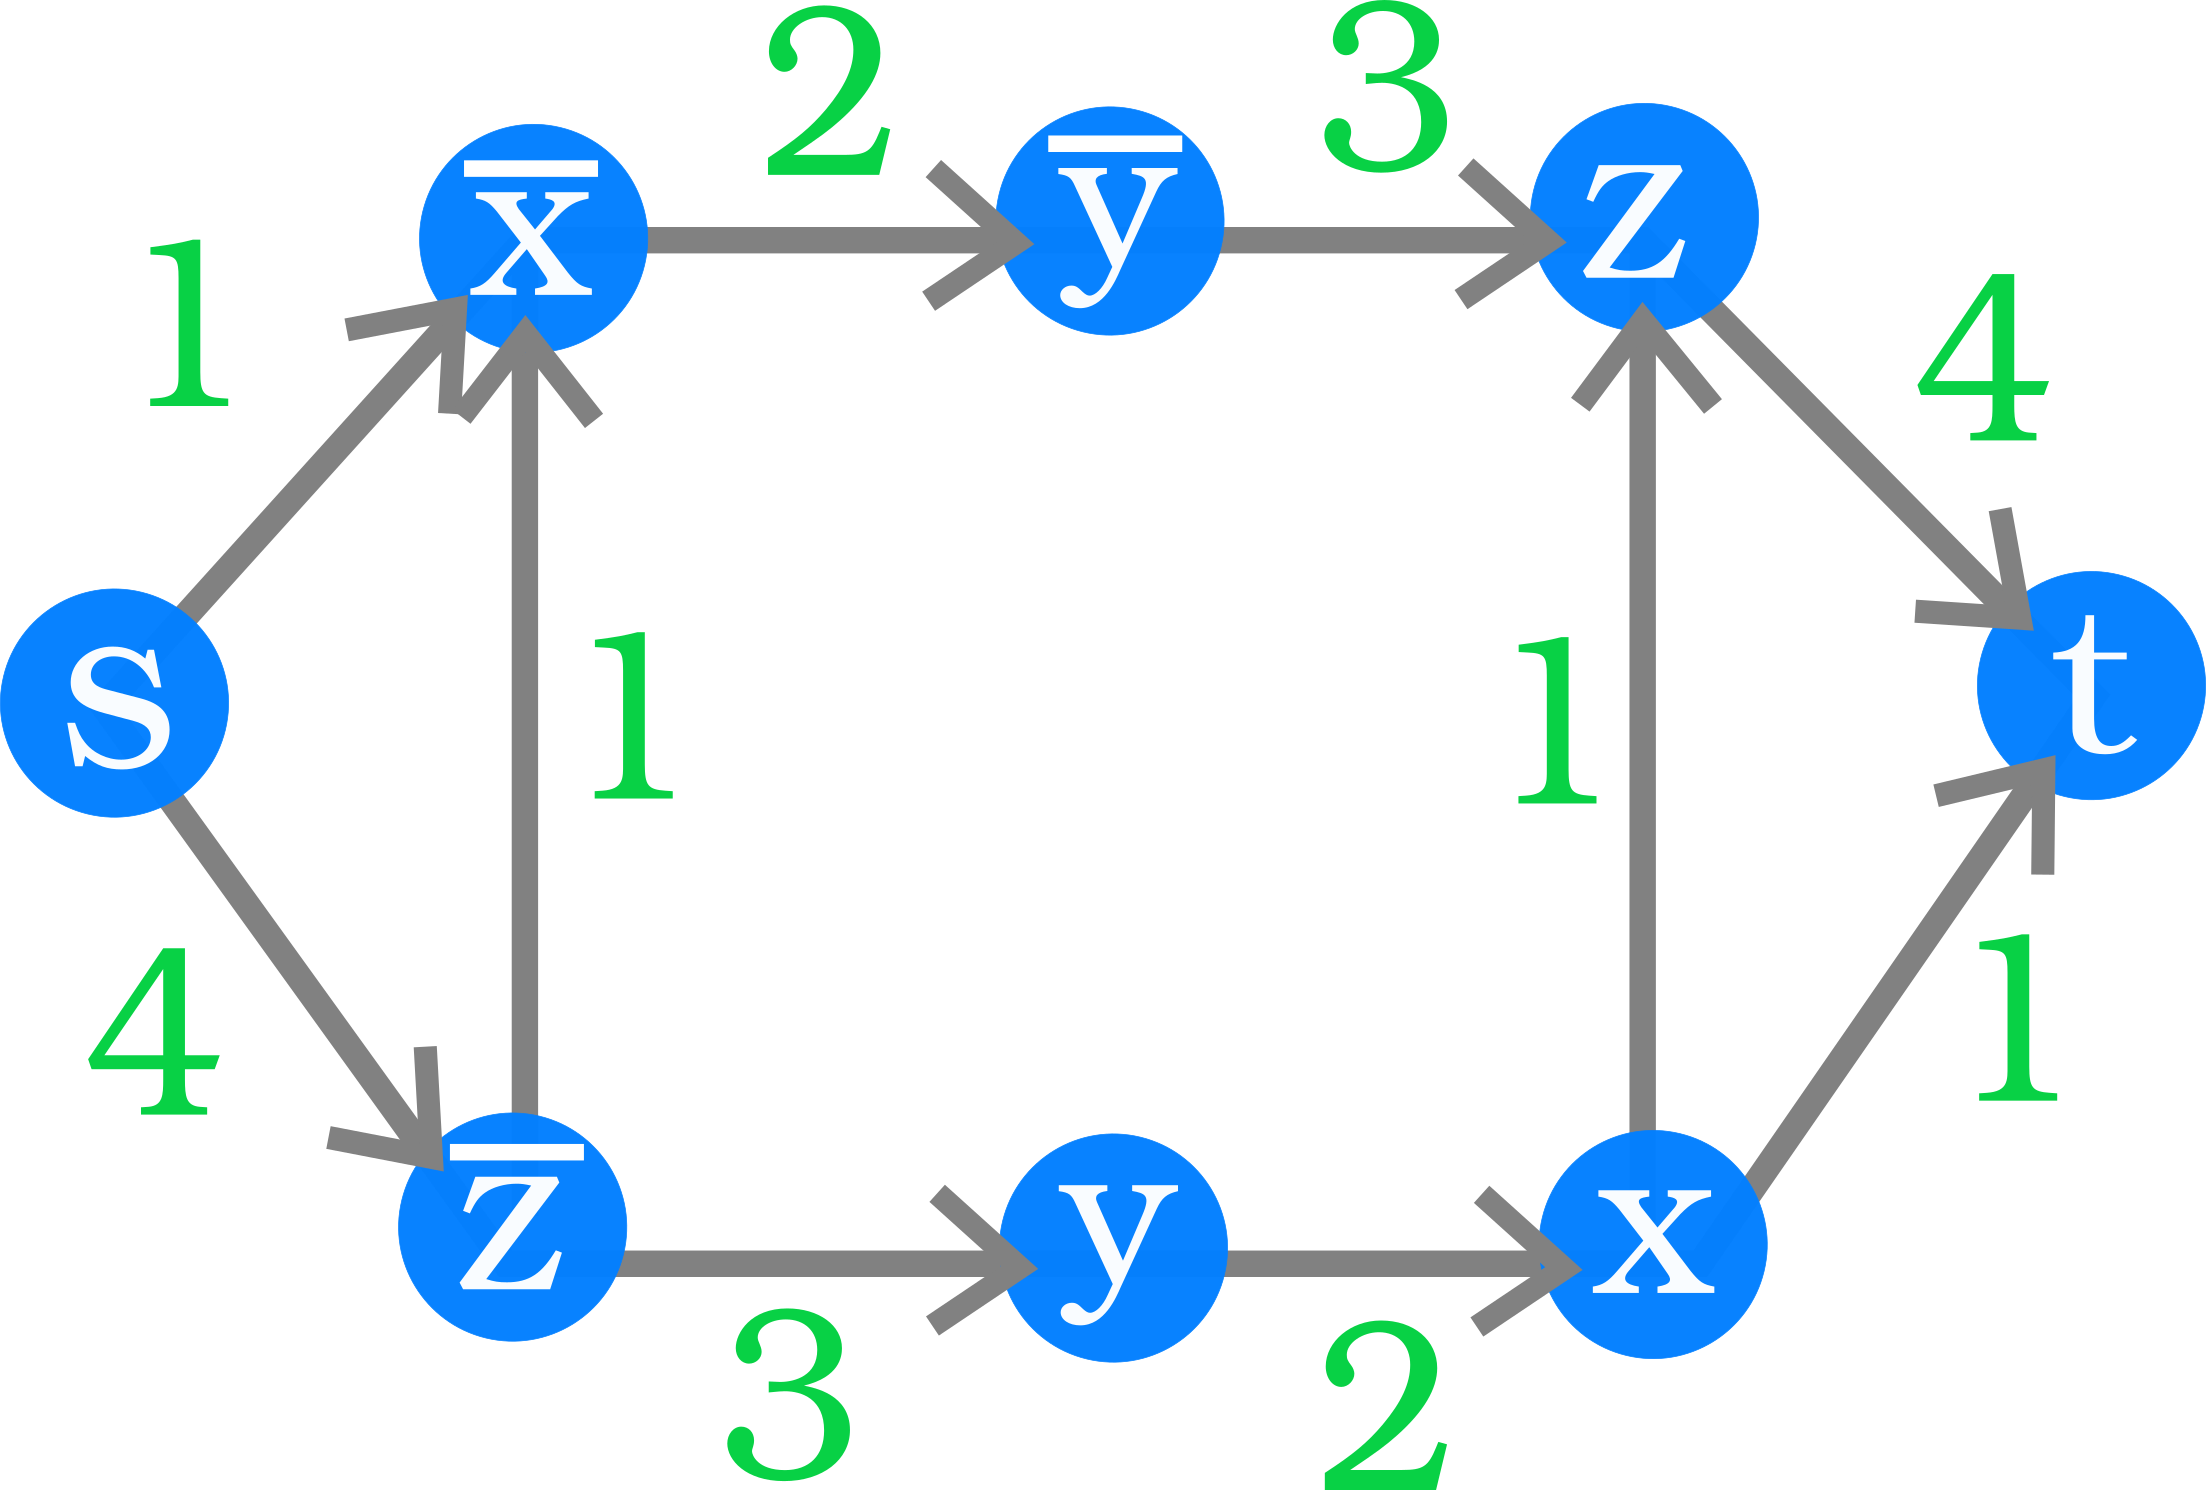
\includegraphics[scale=0.1]{figures/chapter2/master-posiform/posiform-graph-1.png}
}\\
\subfloat[$1$-Augmenting path $1$]{
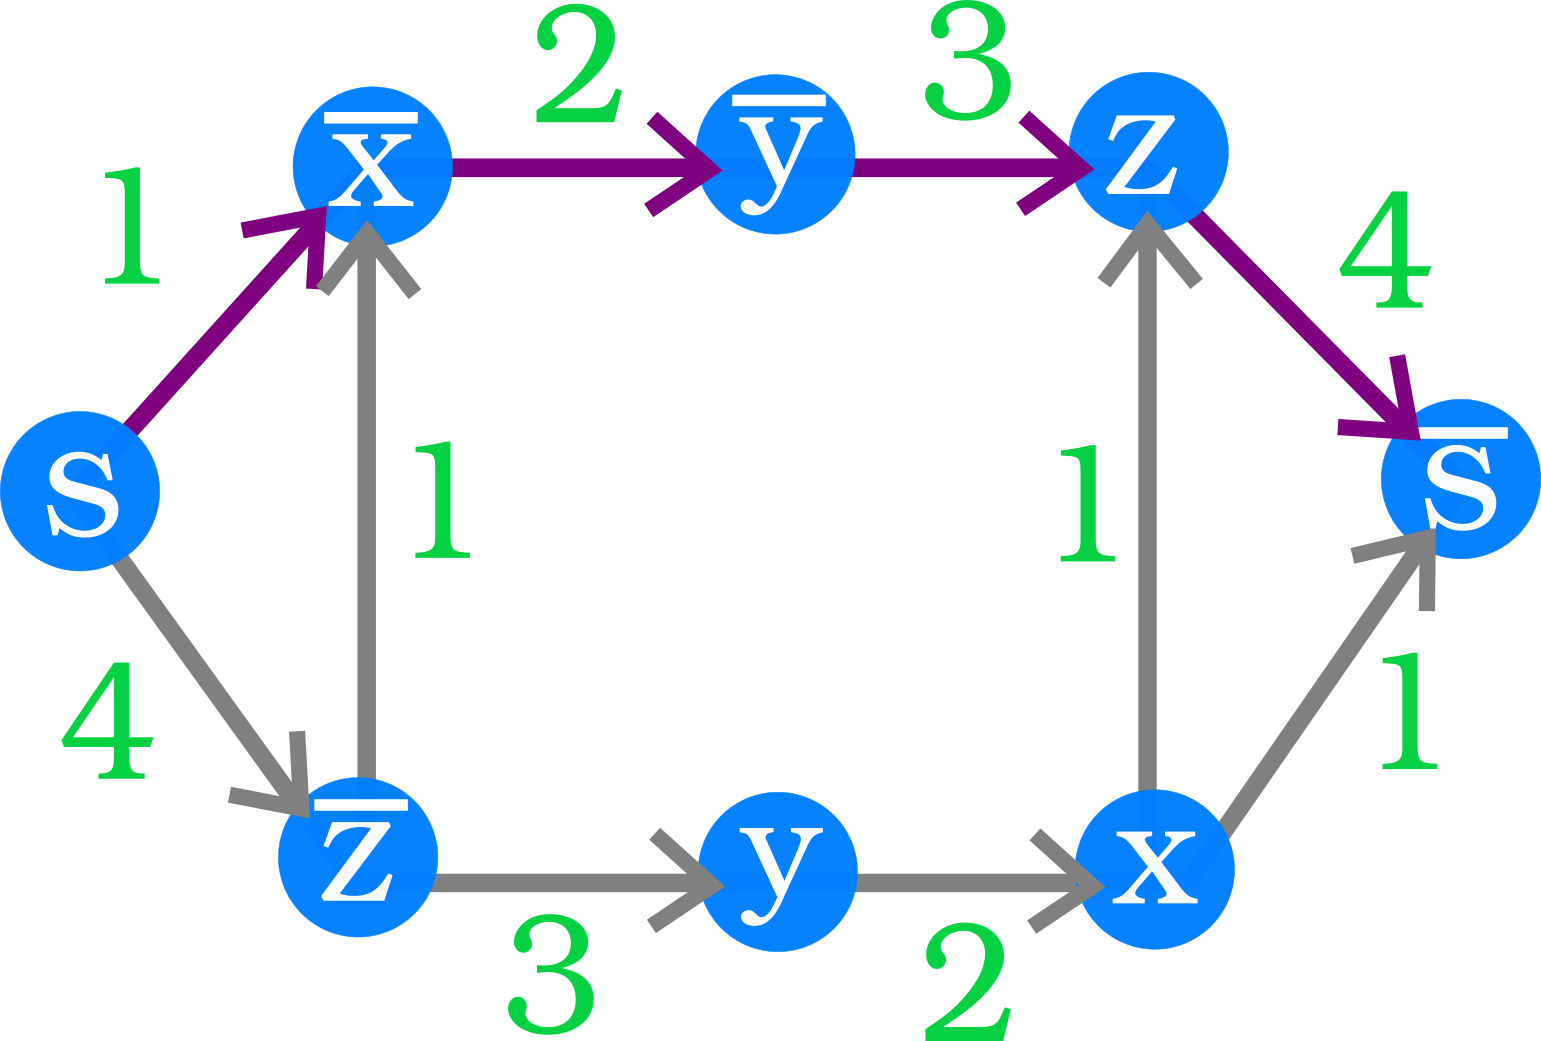
\includegraphics[scale=0.1]{figures/chapter2/master-posiform/posiform-graph-2.png}
}%
\subfloat[$1$-Augmenting path $2$]{
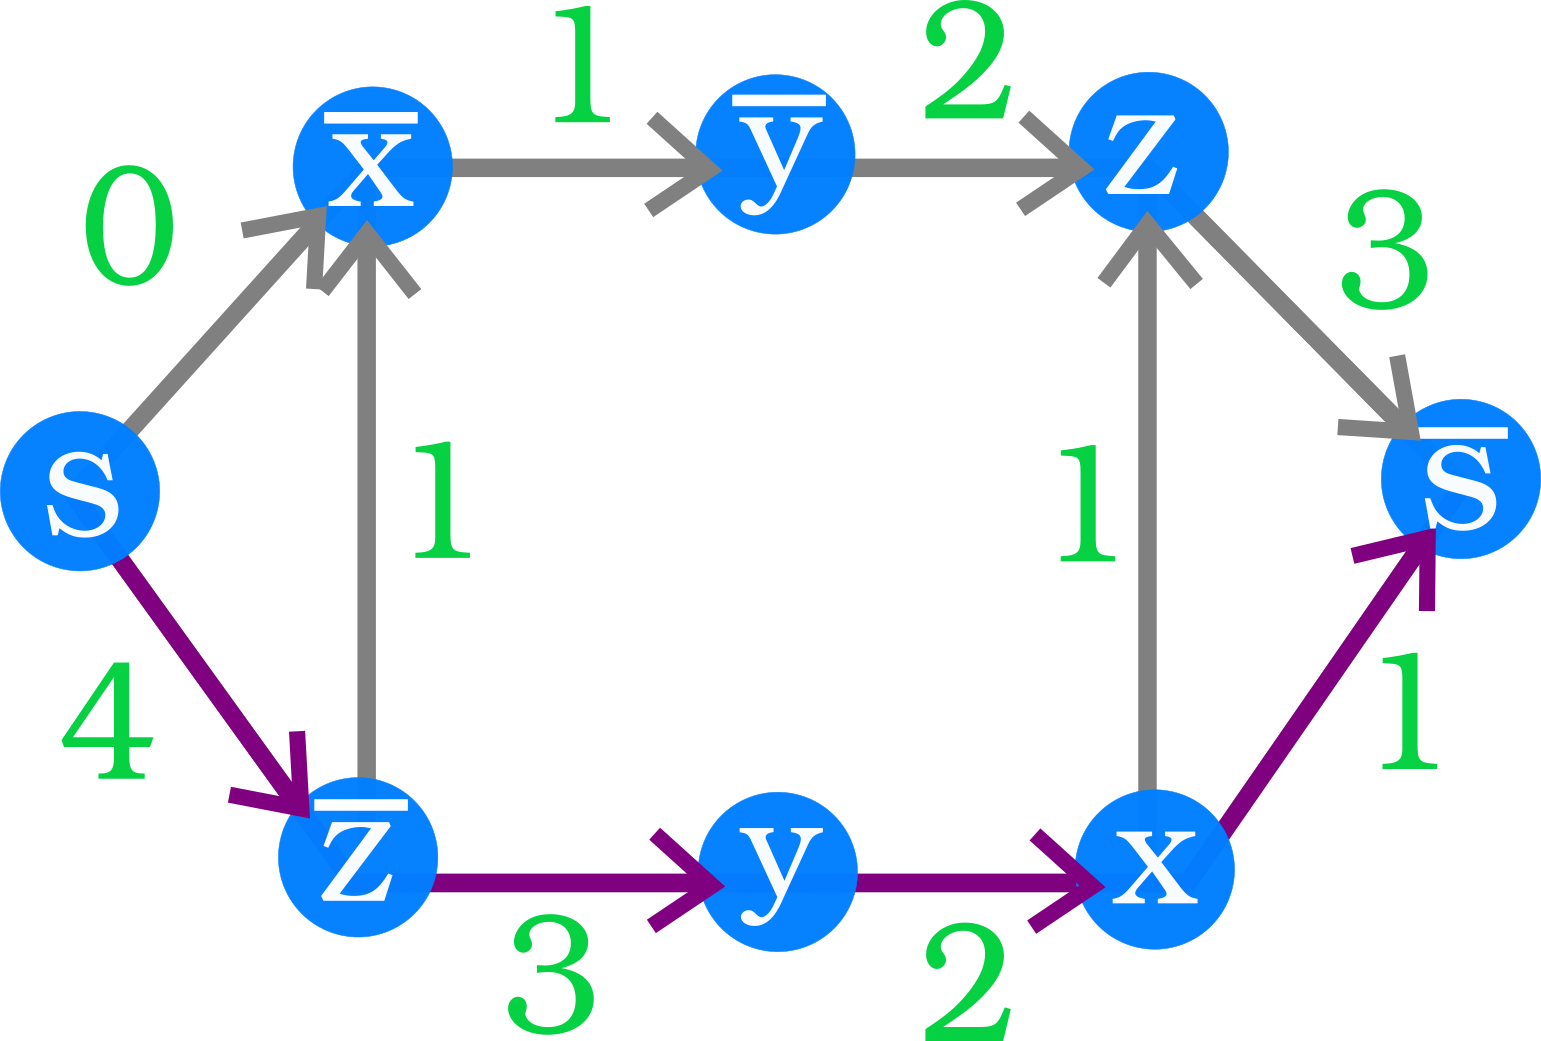
\includegraphics[scale=0.1]{figures/chapter2/master-posiform/posiform-graph-3.png}
}\\%
\subfloat[$1$-Augmenting path $3$]{
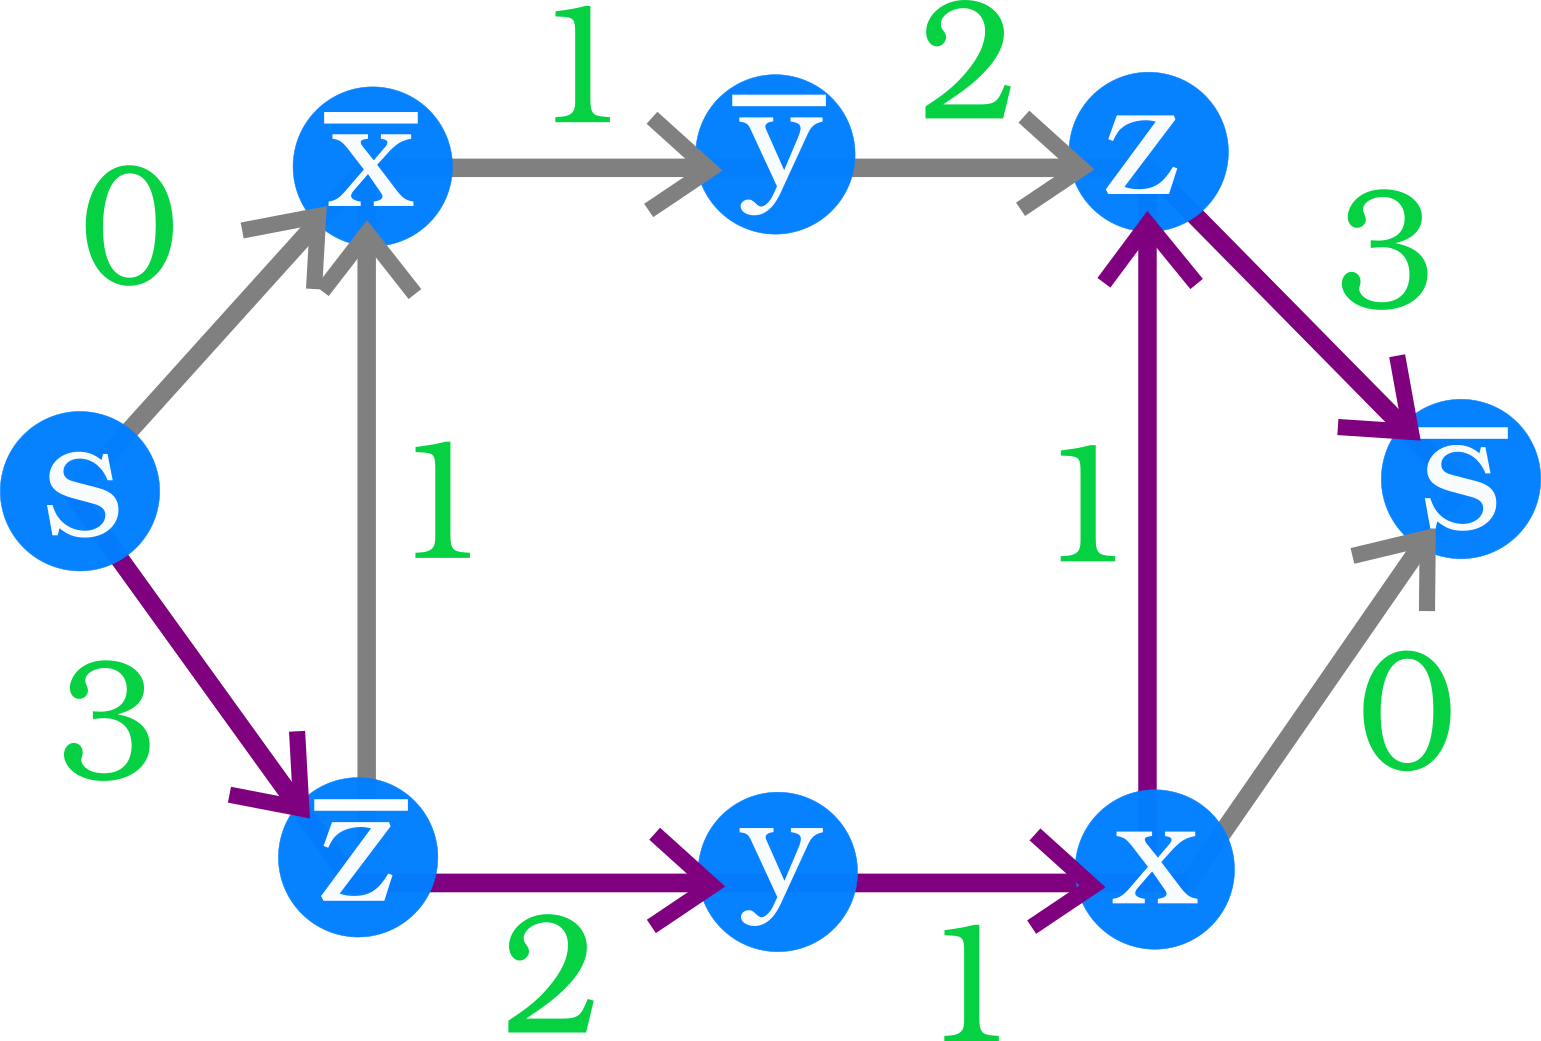
\includegraphics[scale=0.1]{figures/chapter2/master-posiform/posiform-graph-4.png}
}%
\subfloat[$1$-Augmenting path $4$]{
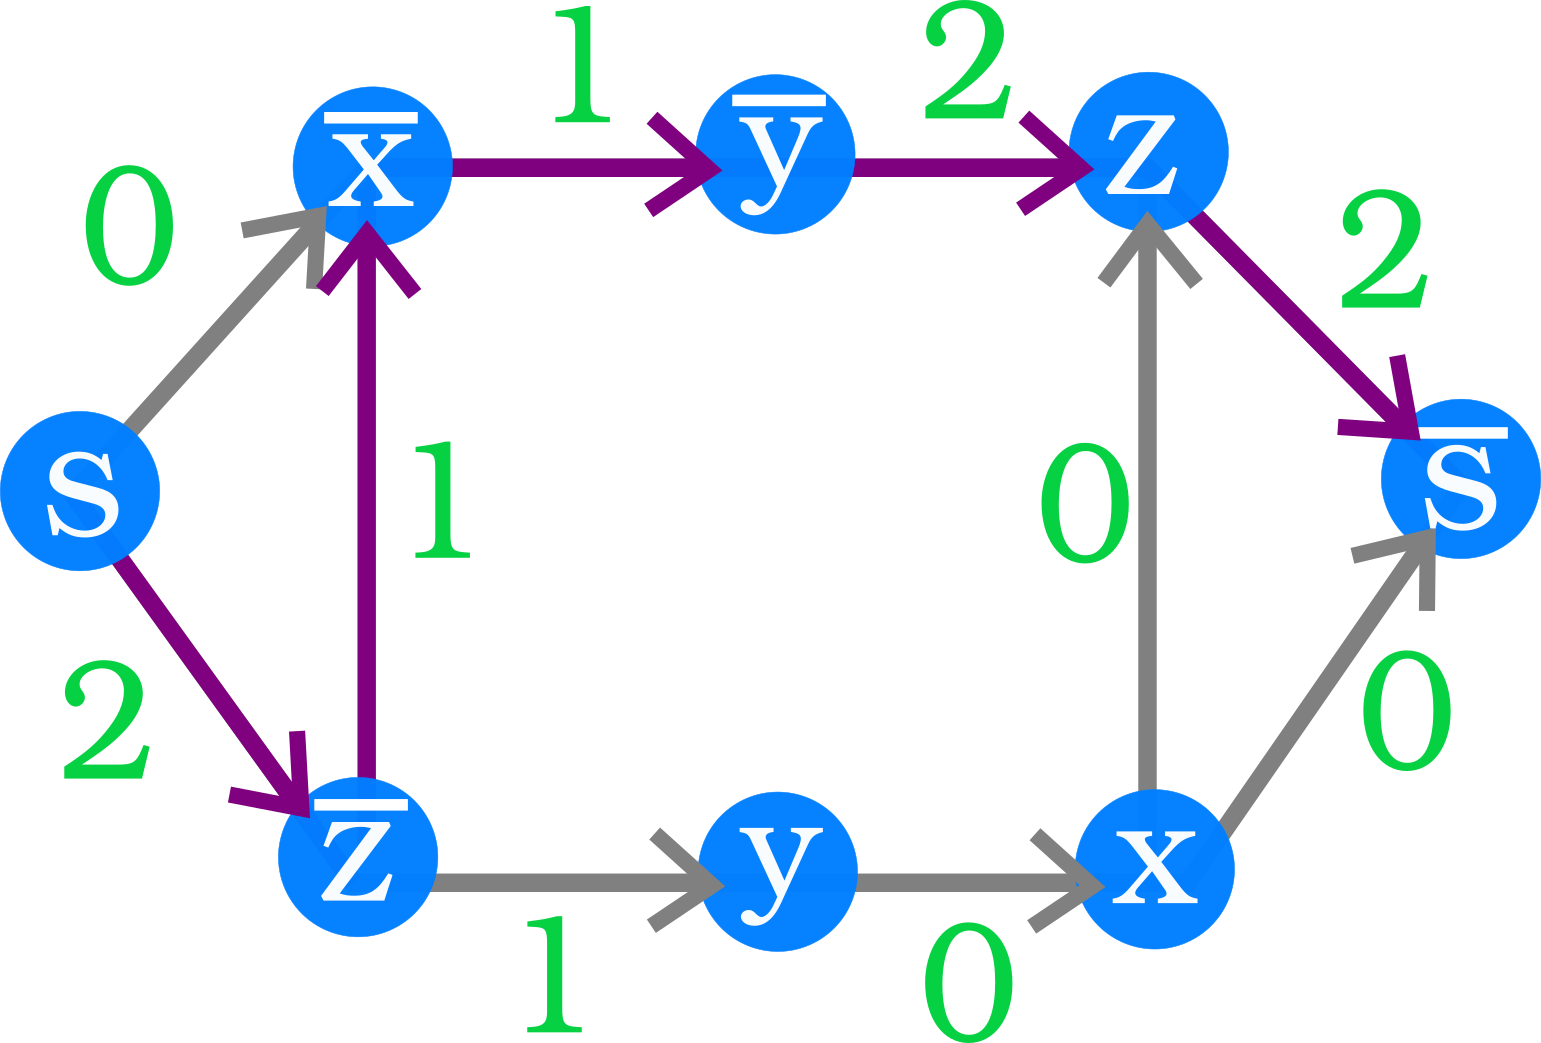
\includegraphics[scale=0.1]{figures/chapter2/master-posiform/posiform-graph-5.png}
}\\%
\subfloat[Final residual graph $G_{ \phi {[\varphi^{\star}]} }$. The master posiform is written as $ { \phi^{\star} } = 4 + 2z +2\bar{z}\bar{y} + 4zy + 4\bar{y}x + 2z\bar{x}$]{
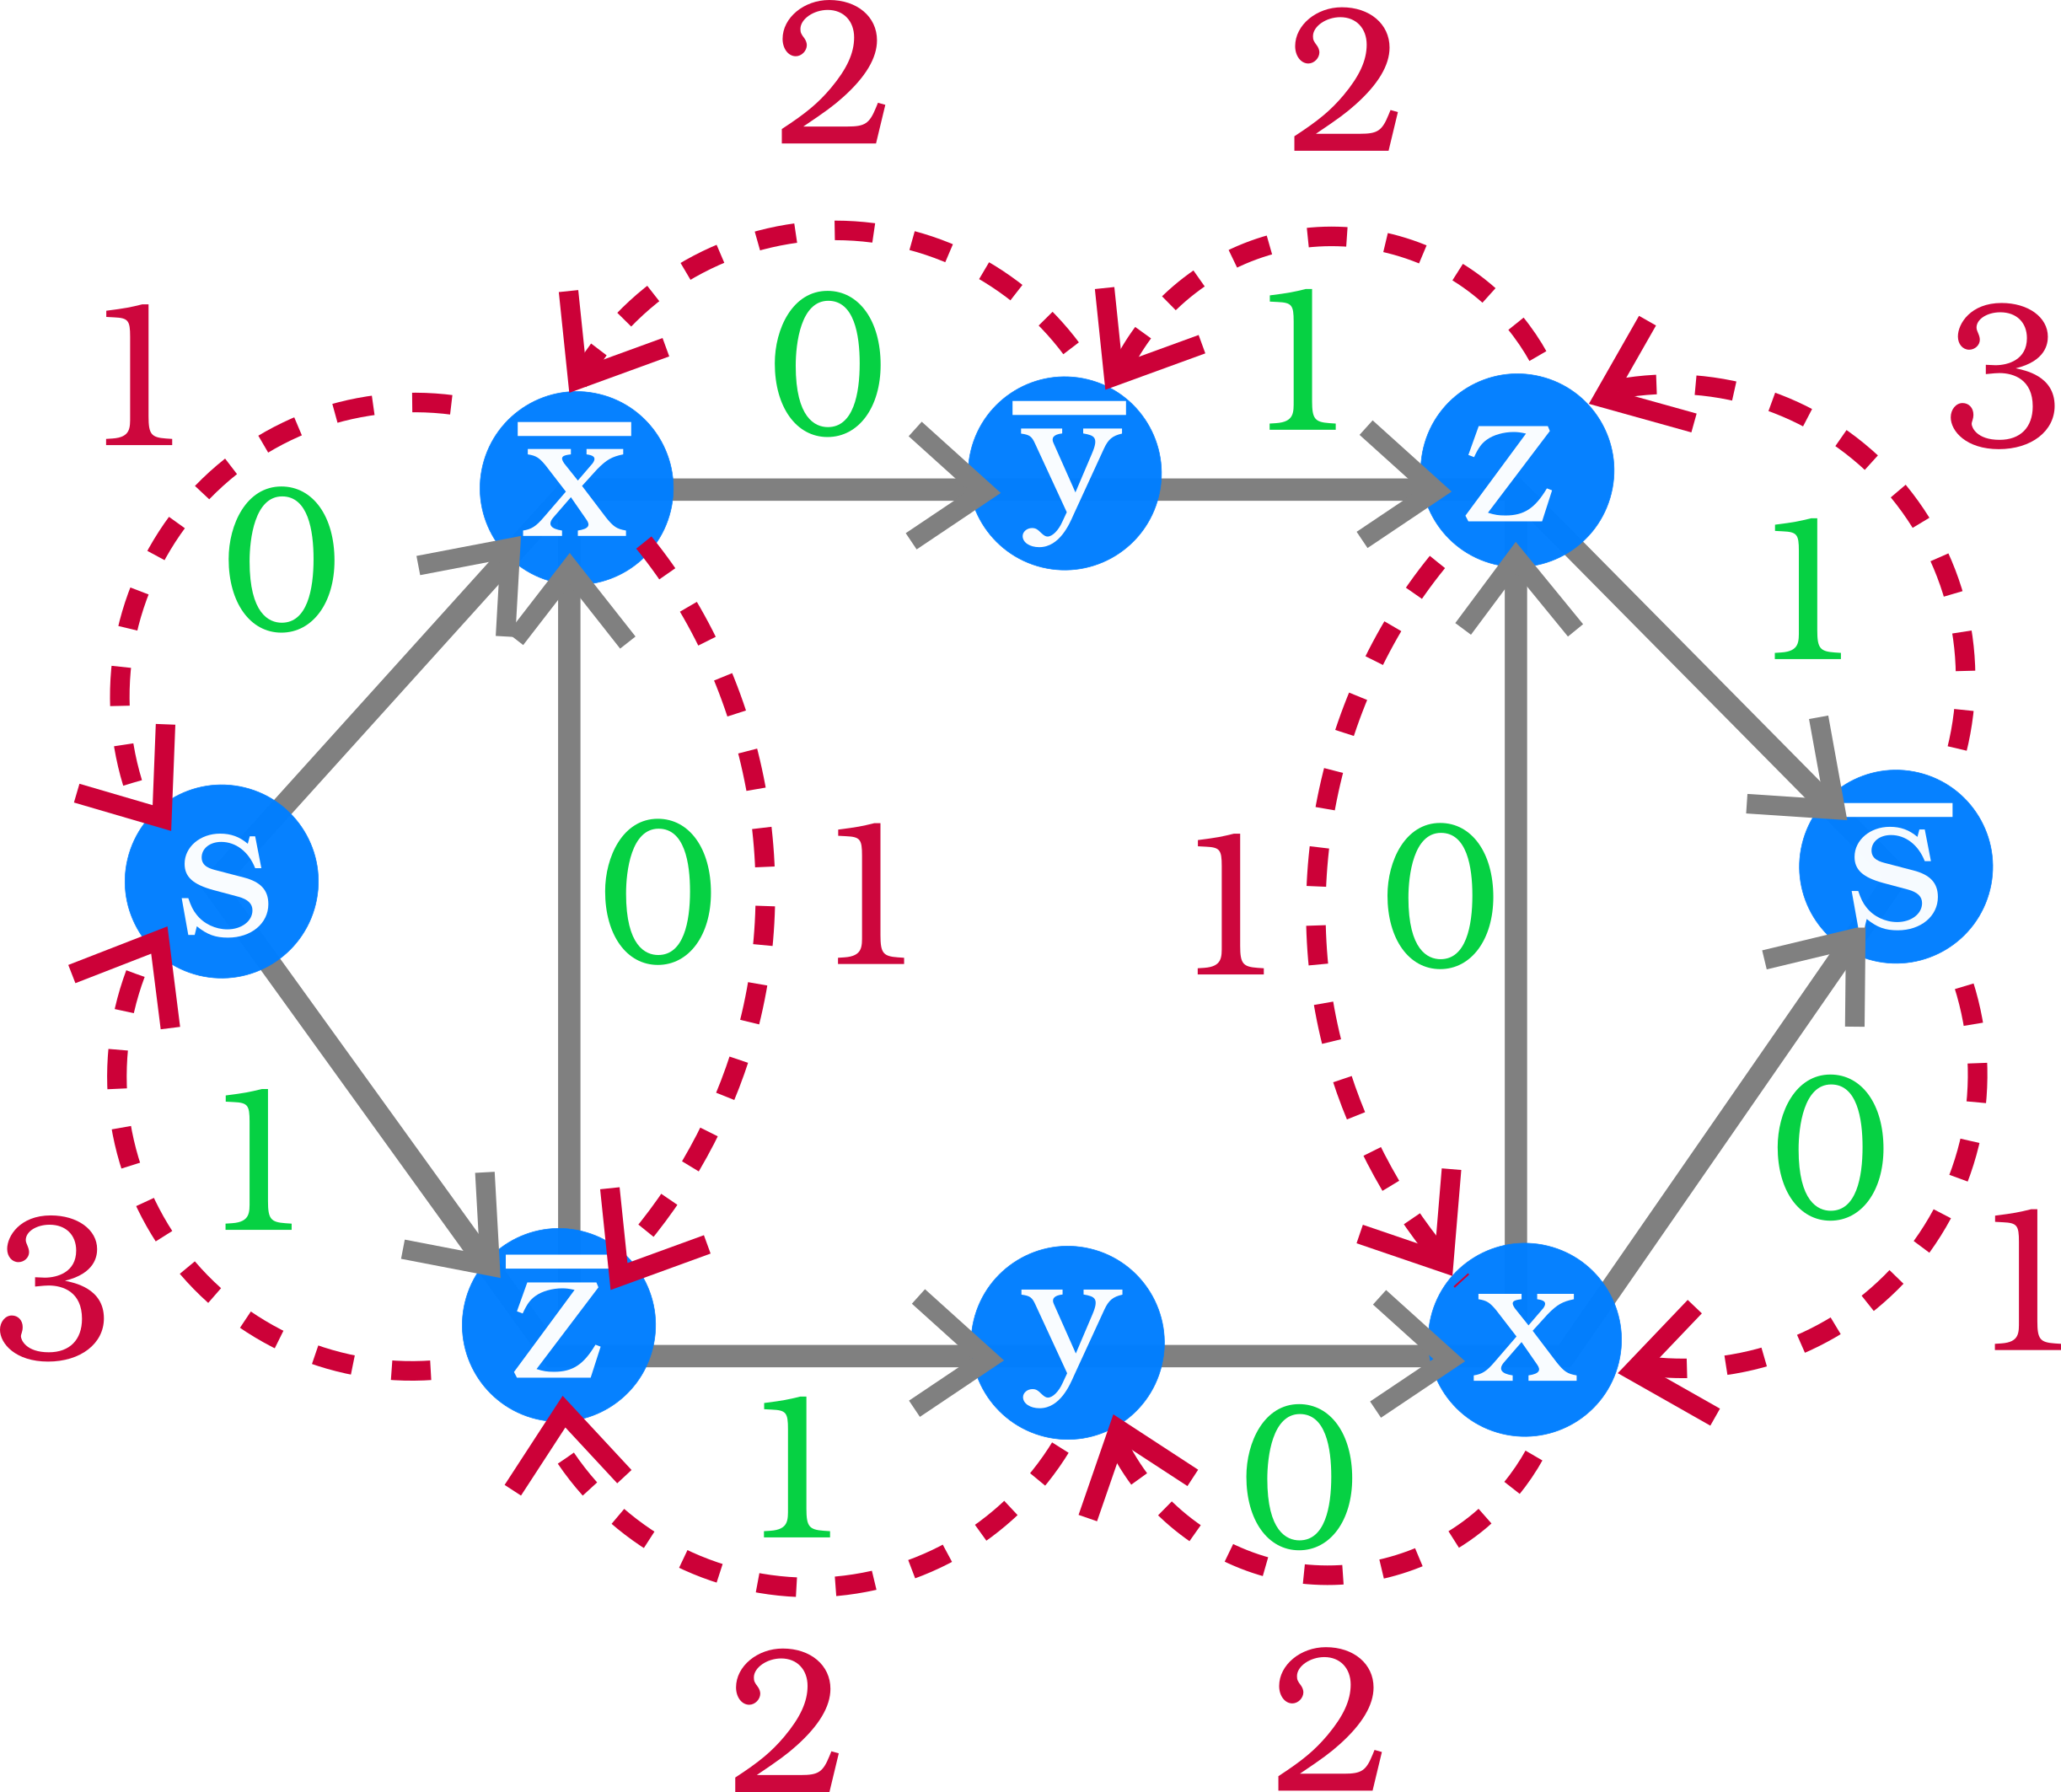
\includegraphics[scale=0.1]{figures/chapter2/master-posiform/posiform-graph-6.png}
}%
\caption{\textbf{Example of max-flow to find the master posiform}. The Ford Fulkerson algorithm is executed for the capacitated graph representation of posiform $\phi$. In~(a), the initial capacitated graph; a sequence of augmenting paths (we omit the returning edges) are shown in figures~(b-e); the final residual graph is shown in figure~(f).  }
\label{ch2:fig:posiform-capacitated-graph}
\end{figure}
%
\begin{proposition}{Residual graph to posiform}
	Given a posiform 
	\begin{align*}
		\phi = C(\phi) + \sum_{p \in L}{a_pp} + \sum_{p,q \in L}{a_{pq}pq},
	\end{align*}
	
	construct its corresponding capacitated graph $G_{\phi}$ and compute its maximum flow executing the Ford Fulkerson algorithm. Then, for every step $k$ of the algorithm we have that
	\begin{align*}
		\phi &= C(\phi) + \nu(\varphi_k) + \phi_{ G_{ \phi [\varphi_k]}}.
	\end{align*}
\end{proposition}
%
\begin{proof}

We observe that every $\epsilon$-augmenting path $\pi_k = s,v_{p_1},v_{p_2},\cdots,v_{p_n},\bar{s}$ in $G_{\phi [\varphi_k]}$ encodes an alternating sum of literals of the form
\begin{align*}
	\phi_{\pi_k} =& a_1\bar{p}_1 + a_{1\bar{2}}p_1\bar{p}_2 + a_{2\bar{3}}p_2\bar{p}_3 + \cdots + a_{n-1\bar{n}}p_{n-1}\bar{p}_k + a_np_n \\
	=&\epsilon( \bar{p}_1 + p_1\bar{p}_2 + p_2\bar{p}_3 + \cdots + p_{n-1}\bar{p}_n + p_n ) + \phi ',
\end{align*}
%
where
\begin{align*}
	\phi ' &= (a_{\bar{1}}-\epsilon)\bar{p}_1 + (a_{1\bar{2}} - \epsilon) p_1\bar{p}_2 + (a_{2\bar{3}}  - \epsilon)p_2\bar{p}_3 + \cdots + (a_{n-1\bar{n}} - \epsilon)p_{n-1}\bar{p}_n + (a_n -\epsilon)p_n.
\end{align*}
%
By observing that
\begin{align*}
	\bar{p}_1 + p_1\bar{p}_2 &= 1 - p_1p_2 \\
	-\bar{p}_{j-1}p_{j} + p_j\bar{p}_{j+1} &= \bar{p}_{j-1}p_j - p_jp_{j+1} \\
	-p_{n-1}p_n + p_n &= \bar{p}_{n-1}p_n,
\end{align*}
%
we can rewrite the alternating sum as
\begin{align*}
	\phi_{\pi} &= \epsilon + \epsilon( \bar{p}_1p_2 + \bar{p}_2p_3 + \cdots + \bar{p}_{n-1}p_n ) + \phi ' \\
	&= \psi + \phi ',	
\end{align*}
%
Note that $\phi '$ and $\psi$ corresponds, respectively, to the update of the residual costs for the edges of $\pi_k$ and the updates of its returning edges. Therefore, we can write
\begin{align*}
	\phi &= C(\phi) + \nu(\varphi_k) + \phi_{ G_{ \phi [\varphi_k] }},
\end{align*}
%
i.e., the initial posiform $\phi$ can be rewritten as a constant plus the posiform corresponding to the residual graph at step $k$ of  the Ford Fulkerson algorithm. 
\end{proof}
%
It follows that the master posiform is given by
\begin{align*}
	\phi^{\star} &= C(\phi) + \nu(\varphi^{\star}) + \phi_{ G_{ \phi [ \varphi^{\star}] }}.
\end{align*}
%
\begin{example}
The posiform $\phi = 2x + 8z + 2x\bar{z} + 4\bar{x}y + 6\bar{y}\bar{z}$ is represented by the graph $G_{\phi}$ in~\cref{ch2:fig:posiform-capacitated-graph}. Its maximum flow value  equals to $4$ and the master posiform is given by $\phi^{\star} = \nu(\varphi ^{\star}) + \phi_{G_{\phi {[\varphi^{\star}}]}} = 4 + 2z + 2\bar{z}\bar{y} + 4zy + 4\bar{y}x + 2z\bar{x}$.
\end{example}
%
From the strong persistency theorem we conclude that $z=0$, and we have
\begin{align*}
	\min \phi = \min \phi^{\star}(z=0) = \min 2\bar{y} + 4\bar{y}x.
\end{align*}
%
We can say more. Let $U$ be the set of literals that are reached from the source by a path of positive residual in the final residual graph. Then, a solution $\vec x \in \argmin f$ must agree with $x(U=1)$~\cite{boros02pseudo}. Therefore,
\begin{align*}
	\min \phi = \min \phi^{\star}(\bar{z}=1,y=1) = \min 4 = 4.
\end{align*}
%
In fact, by looking at all configurations of $\phi$, we observe that $(z=0,y=1)$ in every minimum configuration of $f$.

\begin{center}
\begin{tabular}{|c|c|c|c|}
\hline
$x$ & $y$ & $z$ & $f$\\
\hline
0 & 0 & 0 & 6 \\
0 & 0 & 1 & 8 \\
\textbf{0} & \textbf{1} & \textbf{0} & \textbf{4} \\
0 & 1 & 1 & 12 \\
1 & 0 & 0 & 10 \\
1 & 0 & 1 & 10 \\
\textbf{1} & \textbf{1} & \textbf{0} & \textbf{4} \\
1 & 1 & 1 & 10 \\
\hline
\end{tabular}
\end{center}

The construction above is the core of the \emph{QPBO} algorithm~\cite{boros91} that finds partial solutions of general quadratic PBF. \daniel{The labeled variables by QPBO are guaranteed to belong to an optimum solution. This last property is usually referred as the \emph{partial optimality property} of QPBO, and it is a consequence of the strong persistency theorem.} In the most cases, the master posiform allows us to eliminate only few variables, but if the function $f$ is a \emph{submodular} function, QPBO finds the minimum of $f$.

%The master posiform $\phi^{\star}(f)$ gives us a lower bound for the PBF $f$, which is called the roof dual. In some fortunate occasions, the master posiform allows us to simplify the original optimization problem in a trivial one. That is the case for the class of \emph{submodular} functions.


\subsection{Submodularity}

\begin{definition}{Submodular set function}

Let $V$ be a set with $n$ elements, e.g., $V=\{1,2,\cdots, n\}$. A set function $f:2^V\rightarrow \mathbb{R}$ is submodular if 
\begin{align}
	f(X) + f(Y) \geq f(X \cup Y) + f(X \cap Y),\quad \forall X,Y \subset V.
	\label{ch2:eq:submodular-set-function}
\end{align}
%
\end{definition}
%
An equivalent local definition is given by
\begin{align}
	f(X \cup \{x_1\}) + f(X \cup \{x_2\}) \geq f(X \cup \{x_1,x_2\}) + f(X), \; \forall X \subset V \text{ and } \{x_1,x_2\} \not\subset X.
	\label{ch2:eq:submodular-local}
\end{align}
%
\begin{proposition}{Quadratic submodular PBF}
	Let $f:2^V\rightarrow \mathbb{R}$ a quadratic PBF  written as
	\begin{align*}
		f(x_1,\cdots,x_n) &= C + \sum_{i<n}{f_{i}(x_i)} + \sum_{i<j<n}{f_{ij}(x_i,x_j)}.
	\end{align*}
	Then, the statements below are equivalent
	\begin{itemize}
	 	\item[i]{Function $f$ is submodular.}
		\item[ii]{ $f_{ij}(0,1) + f_{ij}(1,0) \geq f_{ij}(0,0) + f_{ij}(1,1), \quad \forall i<j<n$}
		\item[iii]{ $\frac{\partial^2 f}{\partial x_i\partial x_j} \leq 0, \quad \forall i<j<n$ }
	\end{itemize}
\end{proposition}	
%
	\begin{proof}
	
	\begin{tabular}{rl}
	$\mathbf{(i\rightarrow ii)}$:& Immediately from~\cref{ch2:eq:submodular-local}. \\	
	$\mathbf{(ii\rightarrow iii)}$:&  Writing down the terms in $f$ for variables $x_i,x_j$ we have
	\end{tabular}
	\begin{align*}
		f_{ij}(0,0)(1-x_i)(1-x_j) + f_{ij}(1,1)x_ix_j + f_{ij}(0,1)(1-x_i)x_j + f_{ij}(1,0)x_i(1-x_j).
	\end{align*}
%
	Taking its second derivative
	\begin{align*}
		\frac{\partial^2f}{\partial x_i\partial x_j} &= f_{ij}(0,0) + f_{ij}(1,1) - f_{ij}(0,1) - f_{ij}(1,0) \leq 0.
	\end{align*}
%	
	\begin{tabular}{rl}
		$\mathbf{(iii\rightarrow i)}$:& We define
	\end{tabular}		
		\begin{align*}
			\Delta_{x_i} &= f(x_1,\cdots,x_{i-1},x_i=1,x_{i+1},\cdots,x_n) - f(x_1,\cdots,x_{i-1},x_i=0,x_{i+1},\cdots,x_n) \\
			&= f(X \cup \{x_i\}) - f(X), \quad \text{ where } x_i \notin X.
		\end{align*}		 		
		Therefore
		\begin{align*}
			f( X \cup \{x_1,x_2\}) &= f(X) + \Delta_{x_1} + \Delta_{x_2} + \frac{ \partial^2 f}{\partial x_i \partial x_j} \\
			f( X \cup \{x_1,x_2\}) &= -f(X) + f(X \cup \{x_1\}) + f(X \cup \{x_2\}) + \frac{ \partial^2 f}{\partial x_i \partial x_j}.
		\end{align*}	
%		
		Finally,
		\begin{align*}
			f( X \cup \{x_1,x_2\}) +f(X) - f(X \cup \{x_1\}) - f(X \cup \{x_2\}) &\leq 0.	
		\end{align*}
%		
	\end{proof}

Supermodular functions, on the other hand, are functions that satisfy
\begin{align*}
	f(X) + f(Y) \leq f(X \cup Y) + f(X \cap Y),\quad \forall X,Y \subset V.
\end{align*}
%
Therefore, if $f$ is submodular, $-f$ is supermodular. \daniel{The QPBO algorithm efficiently computes the minimum (maximum) of submodular (supermodular) functions. The opposite problem, i.e., maximizing (minimizing) a submodular (supermodular) function is in $NP$-hard. }

There are functions which are \daniel{neither} submodular \daniel{nor} supermodular and are called \emph{non-submodular}. Optimizing a non-submodular function is in $NP$-hard but QPBO can be used to find a \daniel{partially optimal solution}, as noticed previously.  \daniel{Nonetheless, it is likely the case that QPBO will leave several variables unlabeled while minimizing a non-submodular energy. To attenuate this problem, two variations of QPBO were proposed in~\cite{rother07qpbo}}
\daniel{
\begin{itemize}
	\item[]{\textbf{QPBO-Probe}: Implements a branch-and-bound technique in an attempt to increase the number of variables labeled by QPBO. It keeps the partial optimality property.}
	\item[]{\textbf{QPBO-Improve}: An heuristic that is guaranteed to return a labeling of lower or equal value than the labeling giving by QPBO. The partial optimality property is lost.}
\end{itemize}}
As discussed in~\cref{ch2:sec:markov-random-fields,ch2:sec:pseudo-boolean-functions}, several problems in image processing can be modeled in terms of an HMM $\mathcal{H}$ defined over the image grid graph. The hidden states of $\mathcal{H}$ are often estimated as the maximum likelihood of the induced probability distribution given the set of observed variables $\vec{Y}$. \daniel{In that occasion, we mention that the success of this approach depended on the difficulty of the maximum likelihood computation. We observed that the general problem is NP-Hard for multilabel HMM, and we turn our attention to binary ones. In this case, we have to solve a PBF optimization problem.}

As we have seen, the optimization of a PBF is closely related to the computation of maximum flows, or equivalently, minimum cuts in a graph.\daniel{ In fact, in some applications such as binary segmentation, it is more practical to think in terms of a minimum cut problem than in terms of an HMM one. Both interpretations are equivalent and trigger different insights, but the graph cut mindset fits very nicely in the binary segmentation framework and it gives to us an implicit representation of a digital contour, which can be exploited to incorporate geometric information in the model.} %and  The last interpretation is quite convenient in some applications such as binary segmentation. In fact, to think of the problem as we are going to see in the next section that is more practical to think on the problem as a minimum-cut The cut The HMM machinery can be  as the  a point of view is quite enlightening, as we can interpret problems in imaging with the computation of minimum cuts in its grid graph. In the next chapter we \daniel{describe two models inspired in this idea.}


\section{Graph cut models}
\label{ch2:sec:graph-cut-models}

\daniel{ Graph cut techniques in imaging were pioneered by~\cite{greig89exact} and became popular after the interactive binary segmentation model proposed by~\cite{boykov01graphcut}. In this section, we are going to describe the latter and two other applications of graph cut techniques. The first explains how to set the cost function to estimate perimeter of segmented shapes and the second one extends the first by incorporating a constraint that helps in the segmentation of thin and elongated objects.}

\subsection{Binary segmentation}

Let $\vec{I} \in \mathbb{F}^{m\times n}$ a discrete grayscale image and $\GG (\mathcal{V},\mathcal{E})$ its grid graph. We denote $\vec{x}$ the vector of binary variables indexed by image pixels, i.e., $x_p$ is associated to pixel $p$. We consider the capacitated grid graph $\GGe (\mathcal{V}^+,\mathcal{E}^+,c)$ where 
%It is a binary labeling problem. We present here its formulation as an HMM.
\begin{align*}
	\mathcal{V}^+ &= \mathcal{V} \cup \{s,t\} \\
	\mathcal{E}^+ &= \mathcal{E} \cup \big\{ \{s,v_p\}, \{v_p,t\} \; | \; p \in \vec{I} \big\}.
\end{align*}
The cost function $c$ is defined later. The members of the additional set of edges are referred to as terminal edges. Next, let sets $\mathcal{V}_{fg}, \mathcal{V}_{bg} \subset \mathcal{V}$ to represent foreground and background seeds furnished by the user. A $(s,t)$-cut set of $\GGe$ partitions the graph in connected components $S,T$. The first connected to the source and the other to the target vertex. Vertices in $\mathcal{V}_{fg}$ ($\mathcal{V}_{bg}$) will be forced to be in the source (target) component after the removal of a $(s,t)$-cut set.

The data term is modeled by
\begin{align*}
	\psi_1(x_p) &= \left\{ \begin{array}{ll}
	-\ln  H_{bg}\big( I(p) \big), & \text{if } x_p=0  \\[1em]	
	-\ln  H_{fg}\big( I(p) \big), & \text{if } x_p=1,
	\end{array}\right.
\end{align*}
where $H_{bg},H_{fg}$ are mixed Gaussian distributions derived from foreground and background seeds. We associate the $0$ value to the background label and the $1$ value to the foreground label. The space coherence term is expressed as
\begin{align*}
	\psi_{2}(x_p,x_q) &= \left\{ \begin{array}{ll}
	\displaystyle \exp{ \left(- \frac{1}{d_E(p,q)}\frac{(I(p) - I(q))^2}{2\sigma^2} \right) }, & q \in \mathcal{N}_k(p) \\[1em]
	0, & \text{otherwise},
	\end{array}\right.
\end{align*}
%
where $d_E(p,q)$ is the Euclidean distance between the pixel coordinates of $p,q$ %and $\lambda$ is the parameter to control the influence of the terms in the energy. 
.The value $\sigma$ is interpreted as a parameter to configure the noise level of the input image; and $k$ denotes the chosen neighborhood cardinality of the graph (e.g. $8$).

Finally, given weights $\gamma_r \geq 0$ and $\gamma_b \geq 0$, we define the cost function $c:\mathcal{E}^+\rightarrow \mathbb{R}$ as

\begin{table}[h]
\center
\setlength{\extrarowheight}{0.75em}
\begin{tabular}{|c|c|l|}	
\hline
	\multicolumn{1}{|c|}{\textbf{edge} $\mathbf{e}$} & \multicolumn{1}{c|}{$\mathbf{c(e)}$} & \multicolumn{1}{c|}{\textbf{for}}\\
	\hline
	$\{v_p,v_q\}$ & $\gamma_b \cdot \psi_{2}(x_p,x_q)$ & $\forall p \in \vec{I} \text{ and } q \in \mathcal{N}_k(p)$\\
	\hline
	\multirow{3}{*}{ $\{v_p,s\}$ } & $\gamma_r \cdot \psi_1(x_p=0)$ & $\forall p \in \vec{I} \text{ and } p \notin \mathcal{V}_{fg} \cup \mathcal{V}_{bg}$\\
	& $M$ & $p \in \mathcal{V}_{fg}$ \\
	& $0$ & $p \in \mathcal{V}_{bg}$\\
	\hline
	\multirow{3}{*}{ $\{v_p,t\}$ } & $\gamma_r \cdot \psi_1(x_p=1)$ & $\forall p \in \vec{I} \text{ and } p \notin \mathcal{V}_{fg} \cup \mathcal{V}_{bg}$\\
	& $0$ & $p \in \mathcal{V}_{fg}$ \\
	& $M$ & $p \in \mathcal{V}_{bg}$. \\
	\hline
\end{tabular}
\begin{align*}
\text{where,} \qquad M = 1 + \max_{p \in \vec{I}}{\gamma_b \sum_{q \in \mathcal{N}_k(p)}}{\psi_2(x_p,x_q)}.
\end{align*}
\end{table}

Notice that each vertex in $\mathcal{V}$ must have one and only one of its terminal edges in a cut set. Let $\mathcal{E}'$ be a cut set partitioning $G_{I+}$ in connected components $(S,T)$, the first connected to the source and the other connected to target. Its cut value is written as 
\begin{align}
	E^{gcut}(\GGe,\mathcal{E}') &= \gamma_r \left( \sum_{v_p \in S}{ \psi_1(1) } +\sum_{v_p \in T}{\psi_1(0)} \right) + \gamma_b \sum_{(v_p,v_q) \in \mathcal{E}'}{\psi_2(0,1)}.
\label{ch2:eq:graphcut-cut-value}
\end{align}
%
We observe that~\cref{ch2:eq:graphcut-cut-value} can also be written in the form of the Gibbs energy
\begin{align}
	\gamma_r \sum_{x_p \in \vec{X}}{ \psi_1(x_p) } + \frac{\gamma_b}{2}\sum_{ \substack{x_p,x_q \in \vec{X} \\ x_p \neq x_q }}{\psi_2(x_p,x_q)}.
	\label{ch2:eq:graph-cut-gibbs}
\end{align}
%
%
Therefore, a minimum $(s,t)$-cut of $\GGe$ induces a labeling of minimum value for~\cref{ch2:eq:graph-cut-gibbs}. Vertices connected to the source component of the cut are labeled as foreground and those connected to the target are labeled as background. This interpretation is quite natural for the binary segmentation problem, as a minimum $(s,t)$-cut of the grid graph gives a binary partition of the image. In this sense, one could abstract the HMM machinery underneath and simply construct a graph such that its minimum cut separates the desired objects.

\begin{figure}
\center
\subfloat{
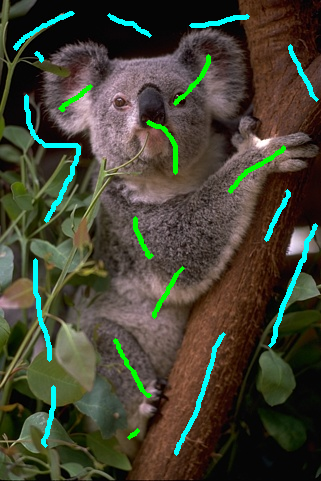
\includegraphics[scale=0.25]{figures/chapter2/grabcut/coala/seeds.png}
}
\subfloat{
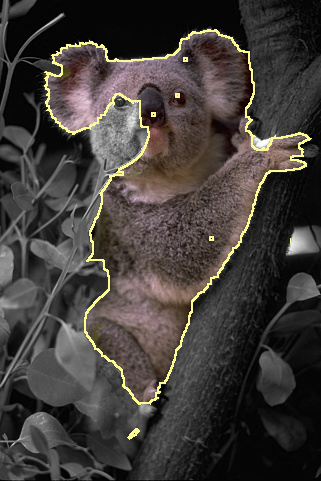
\includegraphics[scale=0.25]{figures/chapter2/grabcut/coala/gc-seg.png}
}\hspace{1em}
\subfloat{
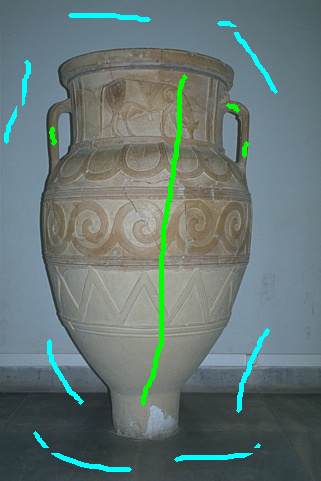
\includegraphics[scale=0.25]{figures/chapter2/grabcut/vase/seeds.png}
}
\subfloat{
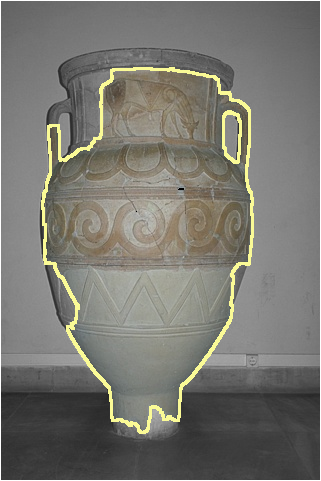
\includegraphics[scale=0.25]{figures/chapter2/grabcut/vase/gc-seg.png}
}
\caption{\textbf{Graph cut segmentation}. Foreground seeds are colored in green and background seeds are colored in blue.}
\end{figure}

Given the particular topology of grid graphs, specific versions of max-flow algorithms were conceived for them. A scalable version of graph cut algorithm~\cite{delong08scalable} can be used for images of high resolution; if several flows should be computed for similar graphs (video sequence segmentation), one can use the flow recycling algorithms~\cite{kohli05efficiently,juan06active}. Although the general complexity of these alternatives may be higher than Ford-Fulkerson algorithm, they are reported~\cite{szeliski06comparative} to compute minimum cuts in lower time for grid graphs.

\subsection{Geodesics computation}

In the previous section, we have seen the natural connection between graph cuts and binary segmentation. The removal of a cut $\mathcal{E}'$ set partitions the grid graph in two disjoint connected components, one connected to the source and associated to the foreground and the other connected to the target and associated to the background. The cut $\mathcal{E}'$ itself can be related with the contour $\partial S$ of the foreground shape (see~\cref{ch2:fig:geodesic-grid-graph-shape-intersection}). In~\cite{boykov03geodesics} it was shown that one can define a cost function for the edge set $\mathcal{E}$ such that the cost of $\mathcal{E}'$ is arbitrarily close to the length of $\partial S$.

The key idea is to use the Cauchy-Crofton formula from integral geometry. In $2D$, let $\mathcal{L}$ be the set of all straight lines in the plane and $d\mathcal{L}$ a Lebesgue measure on this set. Then, the perimeter of a shape $S$ is given by
\begin{align*}
\int_{}{n_c}d{\mathcal{L}} = 2|\partial S|,
\end{align*}
%
where $n_c$ is the number of intersections of some line in $\mathcal{L}$ with the shape contour. To compute the Euclidean length, the cost function should be set as
\begin{align*}
	w_k &= \frac{ \delta^2 \Delta \phi_k }{2 |e_k|},
\end{align*}
%
where $\delta$ is the distance between two lines in the same family and $\Delta \phi_k$ is the angle difference between two consecutive lines (counterclockwise orientation) of different directions in the neighborhood system (see~\cref{ch2:fig:geodesic-grid-graph-shape-intersection}).

\begin{figure}
\center
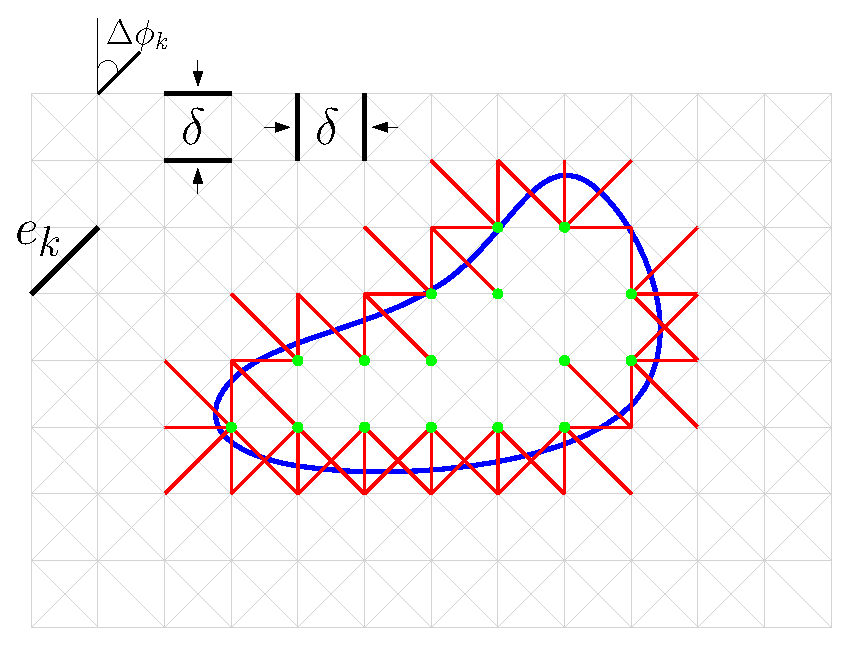
\includegraphics[scale=0.5]{figures/chapter2/perimeter-graph-cuts/geodesics.eps}
\caption{\textbf{Computing perimeter via graph cuts}. The perimeter of a shape $S$ can be encoded as the value of some cut in the grid graph. In the figure, the contour of shape $S$ intersects a set $C \in \mathcal{E}$ of the grid graph with neighborhood system $\mathcal{N}_8$. One can set a cost function on $\mathcal{E}$ such that the cost of $C$ converges to the length of $\partial S$ as the neighborhood system goes to infinity.}
\label{ch2:fig:geodesic-grid-graph-shape-intersection}
\end{figure}

The authors proved equivalent results for an arbitrary Riemannian metric in two and three dimensions. A drawback of this approach is that the quality of the results are very sensitive to the neighborhood system. Small neighborhoods are prone to metrication errors and the convergence theorem, although of theoretical importance, it does not possess the \emph{multigrid convergence} property. The $4$-neighborhood system returns a poor estimation of length no matter the image resolution. We discuss multigrid convergence in~\cref{chapter:digital-geometry}.

Another interesting contribution in the attempt to inject geometric information in the graph cut framework is the connectivity priors of~\cite{vicente08graph}. This work provides an additional tool to the graph cut algorithm in which the user select points of the image that should be connected to the foreground component. An heuristic based on the Dijkstra algorithm for shortest paths is computed using a metric based on the color intensities. The method proved very useful to the segmentation of thin and elongated objects (see~\cref{ch2:fig:graphcut-connectivity}).

\begin{figure}
\center
\subfloat[]{
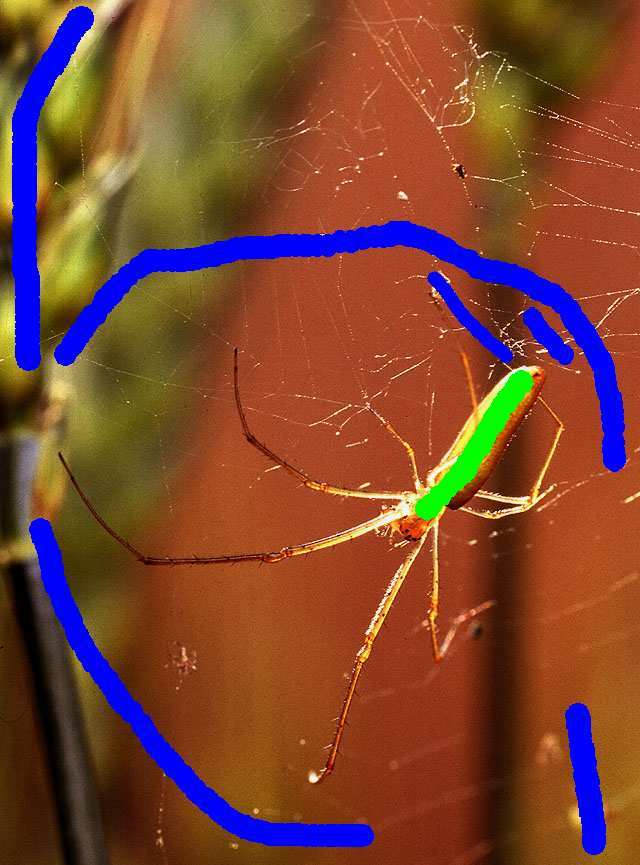
\includegraphics[scale=0.15]{figures/chapter2/grabcut-connectivity/cp-1.png}
}
\subfloat[]{
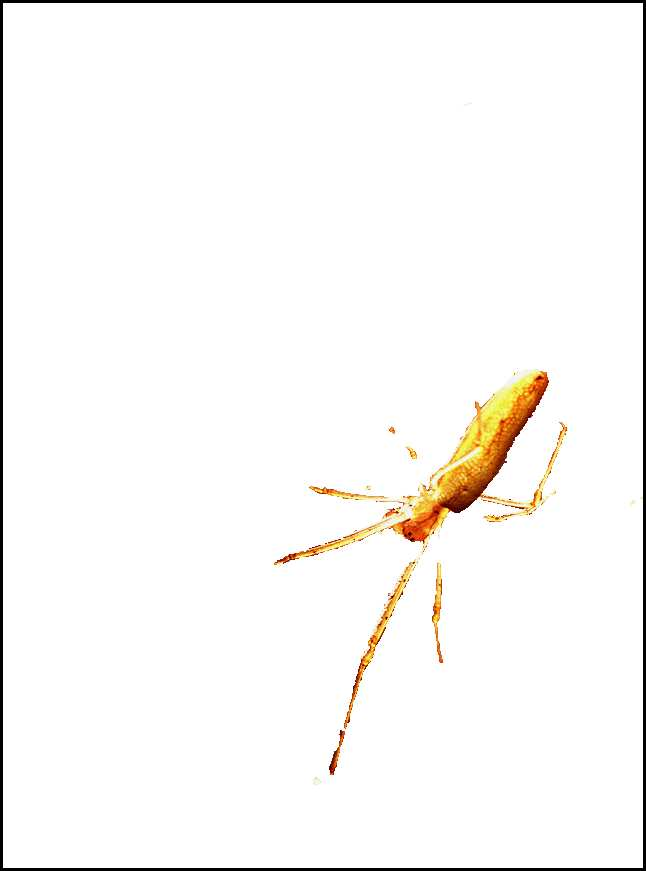
\includegraphics[scale=0.15]{figures/chapter2/grabcut-connectivity/cp-2.png}
}
\subfloat[]{
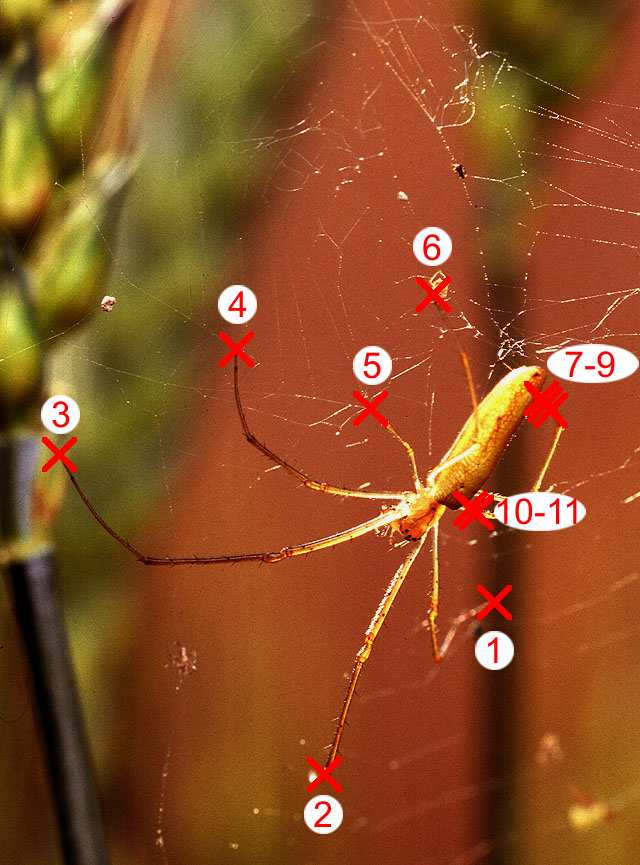
\includegraphics[scale=0.15]{figures/chapter2/grabcut-connectivity/cp-3.png}
}
\subfloat[]{
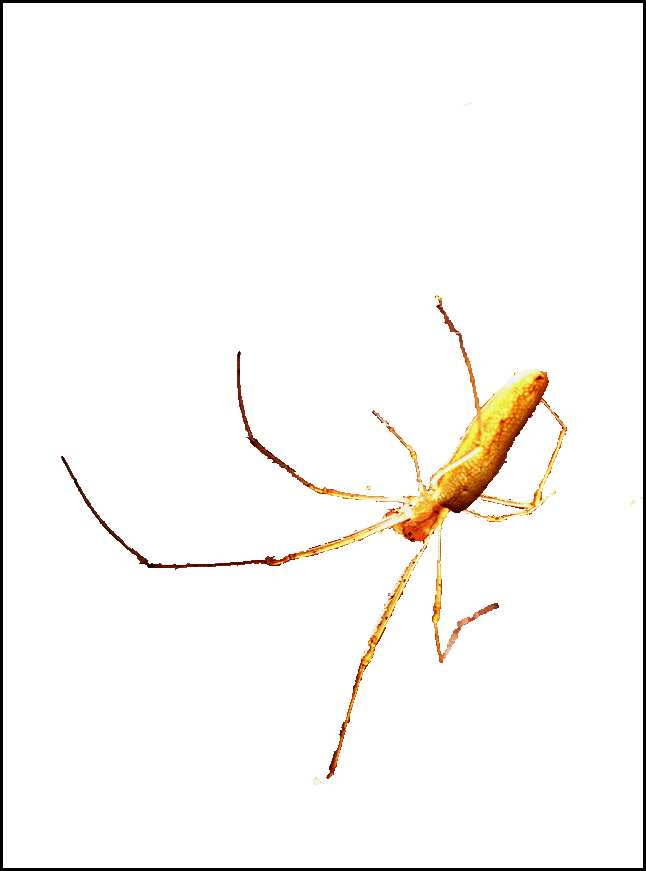
\includegraphics[scale=0.15]{figures/chapter2/grabcut-connectivity/cp-4.png}
}
\caption{\textbf{Graph cut with connectivity priors}~\cite{vicente08graph}. In (a) the foreground (green) and background (blue) seeds. In (b) the graph cut segmentation. In (c) the points selected by the user in which the connectivity constraint is going to be applied. In (d) the final segmentation. }
\label{ch2:fig:graphcut-connectivity}
\end{figure}


%\subsubsection{Approximating multilabel energies with $\alpha$-expansion and $(\alpha,\beta)$-swap}
%
%For pseudo-boolean functions (binary labels), we know that the submodular class is minimized in polynomial time. For energies of order at most three, the problem is reduced to the computation of a minimum cut in a capacitated graph. For higher orders, the best algorithm has complexity $O(n^5Q + n^6)$~\cite{orlin09faster}, where $Q$ is the time to evaluate the function being minimized. If the function is not binary (multilabeling problems), things get more complicated.
%
%At first glance, the multilabeling extension does not seem to be an issue, as we can always transform a multilabel problem in a binary one by including as many as $\log |\Gamma_{\vec{X}}|$ new variables. The difficulty is that the resulting energy is likely  non-submodular~\cite{ramalingam08}, and the minimization of a general non-submodular function is in $NP$-hard. In this section we describe two algorithms to approximate the MAP inference of multilabel problems based on local-search.
%
%A standard approach to devise an approximation solution is the so called \emph{local-search} paradigm described in~\cref{ch2:alg:local-search-paradigm}. The local-search paradigm finds a local minimum (maximum) with respect to some given neighborhood $\mathcal{N}$ and an initial solution $x_0$. The difference between the global and optimum solutions is denoted the \emph{optimality gap}. Naturally, a larger neighborhood tends to decrease the optimality gap and may lead to an increase in the running time. In the extreme case, in which all configurations are present in the neighborhood $\mathcal{N}$, the local-search returns the global optimum solution. Therefore, a successful local-search algorithm is the one that has a good compromise between neighborhood size and optimality gap.
%
%\begin{algorithm}
% \LinesNumbered
% \SetKwInOut{Input}{input}\SetKwInOut{Output}{output}
% \SetKwRepeat{Do}{do}{while}%
% \SetKwComment{comment}{//}{}
% 
%  \Input{Function $f$; an initial solution $x^{(0)}$; and a neighborhood $\mathcal{N}$.}
%  \Output{Local minimum solution of $f$ with respect to neighborhood $\mathcal{N}$ and initial solution $x^{(0)}$.}  
%  \BlankLine
%  
% $t \longleftarrow 0$\;
% \Do{$f(x^{(t)}) < f(x^{(t-1)})$}{
% 	$x^{(t+1)} = \displaystyle \argmin_{ x \in \mathcal{N}(x^{(t)})} f(x)$ \tcp*[l]{Local optimization step} \nllabel{ch2:alg:local-search-local-opt-step} 
%	$t \longleftarrow t + 1$\; 	
% }
% \BlankLine
% 
% \caption{Local search paradigm for minimization.}
% \label{ch2:alg:local-search-paradigm}
%\end{algorithm}
%
%Approximation algorithms like iterated conditional moves (ICM)~\cite{besag86} and simulated annealing~\cite{geman84} defines the neighborhood $\mathcal{N}(\vec{I}^{(t)})$ as the set of images that differs in a single pixel from $\mathcal{N}(\vec{I}^{(t)})$. Consequently, a premature stop in a local optimum of lower quality is likely to happen. 
%
%The idea in the \emph{$\alpha$-expansion} and \emph{$(\alpha,\beta)$-swap} algorithms consists in to define a large neighborhood $\mathcal{N}(\vec{I}^{(t)})$ such that finding the best configuration in such neighborhood can be efficiently computed. In order to illustrate some ideas, let's consider once again the Potts model applied to image denoising of a grayscale image $\vec{I} \in \mathbb{F}^{m \times n}$.
%\begin{align}
%	\phi_{pq}(x_p,x_q) &= \left\{ \begin{array}{ll}
%		K,& \text{if } x_p \neq x_q \\
%		0,& \text{otherwise}.
%	\end{array}\right. \label{ch2:eq:potts-model-denoising-bis-1} \\[1em]
%	E(\vec{x}) &= \sum_{p \in \mathcal{V} }{\phi_p(x_p)} + \sum_{(p,q) \in \mathcal{E}}{\phi_{pq}(x_p,x_q)}.	
%	\label{ch2:eq:potts-model-denoising-bis-2}
%\end{align}
%%
%%
%As mentioned before, minimizing~\cref{ch2:eq:potts-model-denoising-bis-1,ch2:eq:potts-model-denoising-bis-2} is NP-hard as long as variables $x_p,x_q$ take values in a set of cardinality greater than $2$. Notice that if we limit the problem to only two labels, let's say $\alpha,\beta$,~\cref{ch2:eq:potts-model-denoising-bis-1,ch2:eq:potts-model-denoising-bis-2} is a submodular PBF (Ising model) and can be minimized in polynomial time. The key is in to define the transformation function 
%\begin{align*}
%	T_{\alpha,\beta}(x_p,c_p) &= \left\{ \begin{array}{rl}
%		\alpha,& \quad \text{if } ( x_p=\alpha \text{ or } x_p=\beta) ) \text{ and } c_p=0,\\[1em]
%		\beta,& \quad \text{if } ( x_p=\alpha \text{ or } x_p=\beta) ) \text{ and } c_p=1,\\[1em]
%		x_p,& \quad \text{otherwise}.
%	\end{array}\right. ,
%\end{align*}
%%
%and the neighborhood
%\begin{align*}
%\mathcal{N}_{\alpha,\beta}(\vec{I}) &= \left\{ \vec{I}' \; | \; \vec{I}'(p) = T_{\alpha,\beta}(\vec{I}(p),\{0,1\}) \quad \forall p \in \vec{I} \right\}.
%\end{align*}
%%
%%
%In the $(\alpha,\beta)$-swap algorithm, the local-optimization step (~\cref{ch2:alg:local-search-local-opt-step} in~\cref{ch2:alg:local-search-paradigm}) is replaced by
%
%\begin{algorithm}[H]
%  \BlankLine
%  
% 	\For{ $(\alpha,\beta) \in \{0,255\}$ }
% 	{
%	 	$y \longleftarrow \displaystyle \argmin_{ y' \in \mathcal{N}_{\alpha,\beta}(x^{(t)})} f(y')$\;
%	 	\If{ $f(y) < f(x^{(t)})$ }
%	 	{
%	 		$x^{(t)} \longleftarrow y$\;
%	 	}
% 	}
% 	
% \BlankLine
%\end{algorithm}
%
%\begin{figure}
%\center
%\subfloat[Original image]{
%
\includegraphics[scale=0.1]{figures/chapter2/move-making/move-making-1.png}
%}%
%\subfloat[Noisy image]{
%
\includegraphics[scale=0.1]{figures/chapter2/move-making/move-making-2.png}
%}%
%\subfloat[$\alpha$-expansion]{
%
\includegraphics[scale=0.1]{figures/chapter2/move-making/move-making-3.png}
%}%
%\subfloat[Range moves]{
%
\includegraphics[scale=0.1]{figures/chapter2/move-making/move-making-4.png}
%}
%\caption{\textbf{$\mathbf{\alpha}$-expansion x range moves}\cite{veksler07graph}.Comparison of $\alpha$-expansion $\big( (\alpha,\beta)$-swap results are similar$\big)$ and range moves for denoising a piecewise smooth image using the truncated convex potential $\phi_2(x_p,x_q) = \min \{ (x_p-x_q)^2,50 \}$. The range move algorithm returns a smoother image than $\alpha$-expansion. }
%\label{ch2:fig:move-making-examples}
%\end{figure}
%
%The $\alpha$-expansion works in a similar way, except that the only movement allowed is to change a label to some other label $\alpha$. In the $(\alpha,\beta)$-swap algorithm the local optimization energy is submodular if
%\begin{align}
%	\phi_{pq}(\alpha,\alpha) + \phi_{pq}(\beta,\beta) \leq \phi_{pq}(\alpha,\beta) + \phi_{pq}(\beta,\alpha) & \quad \forall \alpha,\beta \in \Gamma_{\vec{X}}.
%	\label{ch2:eq:multilabeling-metric}
%\end{align}
%%
%In the case of $\alpha$-expansion, submodularity is ensured if
%\begin{align}
%	\phi_{pq}(\alpha,\alpha) + \phi_{pq}(\beta,\gamma) \leq \phi_{pq}(\beta,\alpha) + \phi_{pq}(\alpha,\gamma) & \quad \forall \alpha,\beta,\gamma \in \Gamma_{\vec{X}}.
%	\label{ch2:eq:multilabeling-semi-metric}	
%\end{align}
%%
%The $\alpha$-expansion and $(\alpha,\beta)$-swap algorithms have good overall performance for models based in the Potts potential. In~\cite{boykov01fast} we can find nice results for stereo. However, they are less appealing if we use a truncated convex $2$-clique potential~\cite{blake11markov}(see chapter 11). In this case, the \emph{range moves} algorithm proposed in~\cite{veksler07graph} is reported to deliver better results.



%Energies $\phi_{pq}$ that are metrics satisfy~\cref{ch2:eq:multilabeling-metric,ch2:eq:multilabeling-semimetric} and energies that are semi-metrics satisfy~\cref{ch2:eq:multilabeling-semi-metric} only. We recall that $\phi_{pq}$ is metric if
%
%
%\begin{align*}
%	\phi_{pq}(\alpha,\beta) \geq 0 & \quad \text{(Non-negative)} \\
%	\phi_{pq}(\alpha,\beta) = 0 \Leftrightarrow \alpha=\beta & \quad \text{(Null value implication)}\\
%	\phi_{pq}(\alpha,\beta) = \phi_{pq}(\alpha,\beta)  & \quad \text{(Symmetric)} \\
%	\phi_{pq}(\alpha,\beta) \leq \phi_{pq}(\alpha,\gamma) + \phi_{pq}(\gamma,\beta)  & \quad \text{(Triangle inequality)}.
%\end{align*}
%
%A semi-metric is any function that satisfy all conditions above, except the triangle inequality. Examples of metric and semi-metric functions
%
%\begin{align*}
%	f(x,y) &= \min{ \big( K,(I(x)-I(y))^2 \big)} \quad \text{semi-metric} \\
%	f(x,y) &= \min{ \big( K,|I(x)-I(y)| \big) } \quad \text{metric} \\ 
%	f(x,y) &= \left\{ \begin{array}{rl}
%		K,& \text{if } x \neq y \\
%		0,& \text{otherwise}.
%	\end{array}\right.  \quad \text{metric}
%\end{align*}


%\section{GraphCut}
%\subsection{Submodular to graph-cut}
%\subsection{Grabcut}
%\subsection{alpha expansion, alfa-beta swap}
%\section{Image denoising}
%\section{Image segmentation}
%	\subsection{Graph-cuts}
%	\subsection{Watersheds}
%	\subsection{Morphology}	
%	\subsection{Thresholding}		
%	\subsection{Wavelets}		
%	\subsection{Corner, edge detection, filters}
%	\subsection{Region adjacenty graph}
%	\subsection{K-means segmentation}	
%	\subsection{Hough transform, parameter space}
%\section{Image inpainting}	
